\documentclass[10pt,a4paper,twocolumn]{article}

% ============================================================
% Packages
% ============================================================
\usepackage[utf8]{inputenc}
\usepackage[T1]{fontenc}
\usepackage{mathptmx}
\usepackage[margin=1.8cm,top=2cm,bottom=2cm]{geometry}
\usepackage{graphicx}
\usepackage{booktabs}
\usepackage{longtable}
\usepackage{amsmath,amssymb}
\usepackage{hyperref}
\usepackage{caption}
\usepackage{subcaption}
\usepackage{float}
\usepackage{enumitem}
\usepackage{url}
\usepackage{natbib}
\usepackage{tabularx}
\usepackage{multirow}
\usepackage{xcolor}
\usepackage{algorithm}
\usepackage{algpseudocode}

\graphicspath{{results/figures/}}

\hypersetup{
    colorlinks=true,
    linkcolor=blue!60!black,
    citecolor=blue!60!black,
    urlcolor=blue!60!black,
}

% Tighten caption spacing
\captionsetup{font=small,labelfont=bf,skip=4pt}

% Compact lists
\setlist{itemsep=1pt,topsep=2pt,parsep=0pt}

% ============================================================
% Document
% ============================================================
\begin{document}

% --- Title + Abstract in full-width single-column block ---
\twocolumn[{%
\begin{center}
{\LARGE\bfseries Machine Learning Approaches for Cricket Score Prediction:\\[2pt]
A Comprehensive Study with Economic Analysis of the Duckworth-Lewis-Stern Method}

\vspace{0.8em}

{\large Rajat Dogra}

\vspace{0.3em}

{\normalsize 2026}
\end{center}

\vspace{0.6em}
\noindent\rule{\linewidth}{0.4pt}
\smallskip

\noindent\textbf{Abstract.}
The Duckworth-Lewis-Stern (DLS) method has served as the official target-revision system in rain-interrupted limited-overs cricket since 1999. Its parametric model relies solely on overs remaining and wickets in hand---an assumption that increasingly misrepresents modern batting dynamics, where T20-influenced strike rates, aggressive openers, and venue-specific pitch conditions substantially alter scoring trajectories beyond what a two-variable exponential curve can capture. This paper investigates whether machine learning can outperform DLS in two tasks: predicting first-innings totals from intermediate match states, and setting revised targets in rain-affected second innings.

We construct a 46-feature pipeline incorporating Elo team ratings, rolling player statistics (window 30 innings), historical venue profiles, and momentum features---all computed in strictly chronological order with no look-ahead. XGBoost, LightGBM, and CatBoost models are trained with Bayesian hyperparameter optimisation (Optuna, 50--100 trials) using a three-way temporal split at match level, with a dedicated calibration set reserved for conformal prediction intervals. A parallel second-innings pipeline explicitly addresses the right-censoring problem inherent to chase data.

CatBoost achieves a 33\% RMSE reduction over DLS on first-innings prediction ($R^2 = 0.618$ vs.\ $0.150$), with statistical significance confirmed by match-level Diebold-Mariano tests ($p < 0.001$, $T = 542$ matches, HAC bandwidth $h=9$). Second-innings models reduce DLS projection RMSE by 47\%. SHAP analysis identifies player batting statistics and DLS-derived features as the strongest predictors. Evaluated on 255 historical rain-affected matches, the ML revised target engine sets targets 9.9 runs higher on average with substantially reduced variance. A surprising finding is that OLS regression on the 46-feature pipeline matches individual gradient boosting models (RMSE 43.34), establishing that the feature engineering pipeline---not model architecture---is the primary driver of improvement over DLS. Walk-forward cross-validation ($K=5$ folds, RMSE $40.96 \pm 2.35$) confirms stable performance across match eras. An economic impact analysis using a decision-theoretic framework quantifies over \$1.27 million in expected prize money at stake per interrupted ICC World Cup semi-final match under DLS accuracy levels.

\smallskip
\noindent\textbf{Keywords:} Cricket, Duckworth-Lewis-Stern, Machine Learning, Score Prediction, XGBoost, LightGBM, CatBoost, Elo Ratings, Conformal Prediction, Diebold-Mariano Test, Economic Impact

\vspace{0.8em}
\noindent\rule{\linewidth}{0.4pt}
\vspace{0.6em}
}]

% ============================================================
\section{Introduction}
\label{sec:intro}
% ============================================================

\subsection{Background and Context}

Cricket is a bat-and-ball sport with origins in 16th-century England that has grown into one of the most popular sports globally, with an estimated 2.5 billion fans worldwide \citep{icc2023}. In limited-overs cricket---comprising One-Day Internationals (ODIs) with 50 overs per side and Twenty20 Internationals (T20Is) with 20 overs per side---each team bats for a fixed number of overs, with the objective of scoring as many runs as possible within their allotment. The team batting second then attempts to surpass the first team's total within their own allotted overs.

A fundamental challenge arises when matches are interrupted by rain or other external factors, requiring a revised target for the team batting second. This scenario demands a mathematically principled method to adjust the target based on the resources (overs and wickets) available to each team under the revised schedule. The Duckworth-Lewis method, introduced in 1997 by Frank Duckworth and Tony Lewis \citep{duckworth1998} and later refined by Steven Stern \citep{stern2016}, has served as the ICC's official method for target revision since 1999. The method, now known as the Duckworth-Lewis-Stern (DLS) method, models cricket scoring as a function of two key resources: overs remaining and wickets in hand. Its elegant parametric formulation earned wide acceptance precisely because it is transparent, explainable, and computationally simple---qualities that regulators and umpires value highly.

Despite its widespread adoption, the DLS method reflects the scoring dynamics of the 1990s. Modern ODI cricket has been transformed by franchise T20 leagues: average first-innings ODI scores climbed from around 230 in the early 2000s to over 280 by the mid-2020s, powerplay scoring rates have surged, and specialist pinch-hitters routinely attack opposition bowlers in a manner that no two-parameter exponential decay model can fully represent. The mismatch between the DLS resource table (calibrated on older data) and modern batting behaviour has motivated a growing body of academic and industrial work seeking data-driven alternatives.

\subsection{The DLS Mathematical Framework}

The DLS method is built upon a parametric model that expresses the expected additional runs a batting team can score as a function of its remaining resources. The core mathematical formulation is:

\begin{equation}
Z(u, w) = Z_0(w) \cdot \left[1 - \exp\left(-b(w) \cdot u\right)\right]
\label{eq:dls}
\end{equation}

\noindent where $u$ is the number of overs remaining, $w$ is the number of wickets already fallen (0--9), $Z_0(w)$ is the asymptotic maximum runs achievable with $w$ wickets lost, and $b(w)$ is the exponential decay parameter governing how quickly resources deplete as overs are consumed.

The resource percentage remaining at any point is calculated as:
\begin{equation}
R(u, w) = \frac{Z(u, w)}{Z(U, 0)} \times 100\%
\end{equation}

\noindent where $U = 50$ is the total overs in an uninterrupted ODI innings. For target-setting purposes, if Team 1 scores $S_1$ runs using resource percentage $R_1$, and Team 2 has resource percentage $R_2$ available due to interruptions, the revised target is:
\begin{equation}
T_2 = S_1 \times \frac{R_2}{R_1}
\end{equation}

When $R_2 < R_1$ (Team 2 has fewer resources), the target is revised downward; when $R_2 > R_1$ (unusual but possible if Team 1 is interrupted), a $G_{50}$ average innings correction is applied.

\subsection{Motivation and Limitations of DLS}

Several deep limitations motivate this investigation. First, the DLS method operates on only two state variables (overs remaining, wickets fallen), discarding an enormous quantity of potentially predictive information: the current run rate, recent boundary frequencies, batting partnerships, team quality, venue historical averages, atmospheric conditions, and match context. This radical information compression means that DLS treats a situation where a team is scoring at 8 runs per over with their best two batsmen at the crease identically to one where they are scoring at 3 runs per over after losing two wickets in the last three overs---an obviously flawed representation of match dynamics.

Second, the DLS resource table was fitted on historical data from a different era of ODI cricket. \citet{mchale2011modelling} showed that the assumption of a universal resource table fails to account for team-specific scoring patterns. \citet{bhattacharya2011revised} demonstrated that the method systematically disadvantages the team batting second in certain scenarios, particularly when wickets fall in clusters early in the innings. \citet{carter2005model} found that the exponential decay model may not accurately reflect death-over scoring, where modern batsmen often accelerate dramatically regardless of wickets remaining. The parametric structure, while elegant, cannot adapt as cricket evolves.

Third, there is an economic fairness dimension. DLS errors in rain-affected tournament matches can eliminate the wrong team from major competitions, redistributing millions of dollars in prize money incorrectly. The infamous 1992 World Cup semi-final scenario (South Africa needing 21 runs off 1 ball under the then-current rule) motivated DLS's original creation; yet DLS itself has since produced controversies in 2003 and 2022 at the highest stakes of world cricket. The $\$100$--$150$ billion annual cricket betting market in India alone creates additional economic incentives for accuracy.

Fourth, the rapid growth of cricket analytics and the explosion of publicly available ball-by-ball match data (over 4,500 matches on Cricsheet.org \citep{cricsheet}) now makes data-driven modelling tractable at unprecedented scale. Modern ensemble methods---XGBoost \citep{chen2016xgboost}, LightGBM \citep{ke2017lightgbm}, CatBoost \citep{prokhorenkova2018catboost}---routinely outperform traditional parametric models on structured data regression tasks, while Explainable AI techniques (SHAP \citep{lundberg2017unified}, LIME \citep{ribeiro2016should}) address the black-box concern that historically limited ML adoption in high-stakes sporting contexts.

\subsection{Research Questions}

This paper addresses eight research questions:

\begin{description}[leftmargin=0em,style=unboxed,noitemsep]
\item[\textbf{RQ1}:] Can machine learning outperform DLS in predicting first-innings totals from intermediate match states in Men's ODI cricket?
\item[\textbf{RQ2}:] How does ML vs.\ DLS performance vary across innings phases (early, middle, death) and wicket states?
\item[\textbf{RQ3}:] Which features most influence ML predictions, and how do they relate to the DLS resource framework?
\item[\textbf{RQ4}:] Can Explainable AI provide interpretable insight into ML predictions?
\item[\textbf{RQ5}:] Can distribution-free conformal prediction intervals provide reliable uncertainty quantification under temporal covariate shift?
\item[\textbf{RQ6}:] Do stacking ensembles and domain-knowledge monotonic constraints improve over individually tuned GBMs?
\item[\textbf{RQ7}:] Are ML performance gains temporally stable, or does concept drift erode the DLS advantage over time?
\item[\textbf{RQ8}:] What are the economic implications of DLS prediction error in distributional fairness and monetary value across ICC member nations?
\end{description}

\subsection{Contributions}

The primary contributions of this work are:

\begin{enumerate}[leftmargin=1.2em]
\item A data-fitted DLS implementation validated against 3,086 real match records, providing a rigorous parametric baseline.
\item A systematic multi-model comparison (XGBoost, LightGBM, CatBoost) with Bayesian hyperparameter optimisation and three-way temporal split.
\item A 46-feature engineering pipeline incorporating Elo team ratings, rolling player statistics, historical venue profiles, and momentum features---all computed strictly chronologically with no look-ahead.
\item A scientifically rigorous statistical testing framework: match-level Diebold-Mariano tests with Newey-West HAC correction, block-bootstrap confidence intervals ($n=5000$), and Model Confidence Set.
\item A seven-group leave-one-out ablation study quantifying the independent contribution of each feature group.
\item Distribution-free conformal prediction intervals (MAPIE) providing finite-sample coverage guarantees for score projections.
\item A second-innings pipeline with explicit treatment of the right-censoring problem (49.2\% censoring rate) including \texttt{is\_censored} labels and selection-bias documentation.
\item The first ML-based revised target engine evaluated on 255 historical D/L-affected matches.
\item Comprehensive SHAP and LIME explainability analysis linking feature importance to cricket domain knowledge.
\item A 55-feature extended pipeline (V3) adding head-to-head statistics, venue-specific toss advantage, match importance, and seasonality---all computed without look-ahead.
\item Walk-forward cross-validation ($K=5$ expanding folds) demonstrating temporal robustness across match eras 2016--2026.
\item A stacking ensemble (Ridge meta-learner on XGB, LGB, CAT predictions) evaluated against individual models and comprehensive baselines.
\item Domain-knowledge monotonic constraints for XGBoost baking in 22 positive and 8 negative physical constraints.
\item A baseline hierarchy (naive, OLS, Ridge, polynomial, DLS, GBM) establishing that feature engineering---not model architecture---drives the DLS improvement.
\item Temporal stability analysis (concept drift) with Pearson trend statistics confirming stable or improving ML performance across the test period.
\item Bonferroni-corrected DM test $p$-values and Cohen's $d$ effect sizes providing stronger statistical guarantees.
\item An economic impact analysis framing DLS as an economic mechanism: Gini-coefficient equity analysis, Expected Value of Information framework, and one-sample $t$-test confirming DLS's statistically significant directional bias.
\end{enumerate}

\subsection{Paper Organisation}

Section~\ref{sec:litrev} reviews the DLS literature, ML in sports analytics, ML in cricket, and explainable AI. Section~\ref{sec:methodology} details the full experimental methodology including data, feature engineering, model architectures, and evaluation framework. Section~\ref{sec:results} presents all experimental results: first innings, second innings, phase-wise, statistical tests, ablation, conformal prediction, baselines, walk-forward CV, stacking, monotonic constraints, and temporal stability. Section~\ref{sec:economics} analyses economic implications: motivating cases, the fairness equity framework, target-setting bias, expected value computations, and policy implications. Section~\ref{sec:conclusion} summarises findings, limitations, and future work.

% ============================================================
\section{Literature Review}
\label{sec:litrev}
% ============================================================

\subsection{The DLS Method: History and Criticism}

The challenge of revising targets in interrupted cricket matches predates DLS. Earlier approaches including the ``Average Run Rate'' method and the ``Most Productive Overs'' method were widely criticised for producing manifestly unfair targets \citep{duckworth1998}. The Average Run Rate method simply prorated the target by the fraction of overs available, ignoring the crucial role of wickets in hand. The Most Productive Overs method, while more sophisticated, penalised the team batting second by requiring them to match the best overs of the first team's innings---an approach that produced the infamous 1992 World Cup scenario.

Duckworth and Lewis \citep{duckworth1998} proposed a fundamentally different approach by modelling the two key resources available to a batting team---overs remaining and wickets in hand---as a combined ``resource percentage.'' Their 1998 paper, published in the Journal of the Operational Research Society, showed that a two-parameter exponential model could explain the majority of variance in historical scoring data and produce fairer targets than all predecessor methods. The ICC officially adopted the method in 1999.

In 2014, Steven Stern introduced significant refinements to the original model \citep{stern2016}. The key innovation was a revised parametric form that better handled high-scoring matches and adjusted for the increasing scoring rates in modern ODI cricket. The ``Professional Edition'' of the DLS method uses a more complex parametric structure with additional parameters fitted to a continuously updated dataset, though the published academic version retains the exponential form. Stern's modifications were particularly motivated by the observation that Twenty20 cricket had altered batting strategies, with players more willing to sacrifice wickets for strike rate---a behaviour the original DLS parameters under-represented.

Despite these refinements, the DLS method has faced substantial academic criticism. \citet{mchale2011modelling} argued that the assumption of a single universal resource table fails to account for team-specific scoring patterns; top-ranked teams systematically outperform the DLS par score at every wicket state, meaning the resource table encodes an ``average'' team that does not represent any individual playing side. \citet{bhattacharya2011revised} demonstrated that the method systematically disadvantages the team batting second in certain scenarios, particularly when wickets fall in clusters---a common pattern in limited-overs cricket where middle-order batting is fragile. \citet{carter2005model} showed that the exponential decay model may not accurately reflect scoring patterns in the death overs, where specialist finishers (Shahid Afridi, MS Dhoni, Hardik Pandya) can score at strike rates above 200 without regard for wickets remaining. More broadly, the DLS method cannot incorporate information about run rates, boundary frequencies, batting partnerships, current batter quality, or contextual factors such as venue pitch character---all of which have strong predictive value for final score.

A directly relevant contribution is \citet{zia2022player}, who propose a player-aware resource compensation model demonstrating that incorporating team history, player identities, and venue substantially improves upon DLS's generic resource table. Critically, they find DLS par score accuracy is as low as 50--60\% in the 20--24 over range (0--2 wickets lost)---the very scenarios where rain interruptions most commonly occur mid-innings. This work validates the ML-vs-DLS comparison direction but does not employ the rigorous statistical testing framework, full second-innings treatment, conformal prediction, or economic impact analysis developed in this paper.

\subsection{Machine Learning in Sports Analytics}

The application of machine learning to sports prediction has grown substantially over the past two decades. \citet{bunker2019machine} provides a comprehensive survey of ML applications across various sports, identifying regression and classification as dominant paradigms. Gradient boosting methods have emerged as the dominant approach for structured data prediction tasks. \citet{chen2016xgboost} introduced XGBoost with $L_1$/$L_2$ regularisation and column subsampling; \citet{ke2017lightgbm} proposed LightGBM with histogram-based splitting and gradient-based one-side sampling; \citet{prokhorenkova2018catboost} introduced CatBoost with ordered boosting to prevent target leakage. These methods have consistently outperformed traditional statistical models in sports analytics benchmarks \citep{bunker2019machine}.

\citet{baboota2019predictive} demonstrated the effectiveness of ensemble methods for football match outcome prediction, achieving accuracies exceeding 60\% by combining gradient boosting with careful feature engineering, highlighting the importance of domain-specific feature construction over raw model architecture. Similarly, \citet{huang2010neural} applied neural networks to baseball run prediction, showing that non-linear models capture complex game-state interactions that linear methods miss. The broader lesson across sports analytics is that domain-informed feature engineering typically delivers larger performance gains than switching between model architectures---a finding that will recur in our baseline hierarchy results.

\subsection{Machine Learning in Cricket}

Cricket analytics has experienced rapid growth. \citet{sankaranarayanan2014auto} developed a Random Forest system for live win probability estimation in cricket using ball-by-ball features. \citet{passi2018cricket} applied neural networks and SVMs to predict ODI match outcomes, achieving accuracies up to 80\%. The task most directly related to our work---predicting the final score from an intermediate state---has received increasing attention.

\citet{jhanwar2016predicting} applied linear regression, SVMs, and Random Forests to ODI score prediction using team-level features, finding that ensemble methods significantly outperformed linear models, though their work used match-level rather than ball-by-ball features, limiting prediction granularity. \citet{viswanadha2017dynamic} proposed a dynamic Bayesian network for cricket score prediction that explicitly modelled dependencies between overs, achieving improvements over DLS in certain scenarios but lacking the feature richness and scale of modern gradient boosting approaches.

\citet{kampakis2015using} argued for the importance of model interpretability in cricket analytics, noting that DLS's acceptance is partly attributable to its transparent parametric structure. This observation underscores the need for any ML alternative to provide comparable interpretability through explainability techniques. A small number of studies have directly compared ML with DLS. \citet{davis2015investigating} compared neural networks with DLS for T20 cricket, finding that neural networks could achieve competitive accuracy, though their study used a relatively small dataset and lacked modern hyperparameter optimisation.

\subsection{Explainable AI in Sports}

The ``black-box'' concern has been persistent in sports analytics, where administrators and regulators require not just accurate predictions but explainable ones. \citet{lundberg2017unified} introduced SHAP (SHapley Additive exPlanations), which provides theoretically grounded feature attributions based on Shapley values from cooperative game theory. SHAP has been particularly successful for tree-based models through the TreeExplainer algorithm \citep{lundberg2020local}, which computes exact Shapley values in polynomial time by exploiting the tree structure. \citet{ribeiro2016should} proposed LIME (Local Interpretable Model-agnostic Explanations), which approximates any black-box model locally with an interpretable linear model, enabling instance-level explanations suited to explaining individual prediction decisions.

\subsection{Research Gap}

Despite this growing literature, several important gaps remain. No existing study provides a comprehensive comparison of multiple state-of-the-art gradient boosting methods against a properly data-fitted DLS baseline using a large-scale, temporally split dataset. Previous comparisons have not employed modern Bayesian hyperparameter optimisation, which is critical for fair model comparison. Phase-wise and wicket-state analysis has not been systematically conducted at scale, leaving gaps in understanding where ML excels versus where DLS remains competitive. The application of SHAP to cricket score prediction is largely unexplored. No prior work has evaluated ML revised targets on a substantial corpus (255 matches) of real historical D/L-affected matches, nor has any study quantified the economic consequences of DLS error through a formal welfare-economics framework. This paper addresses all of these gaps.

% ============================================================
\section{Methodology}
\label{sec:methodology}
% ============================================================

\subsection{Data Collection and Processing}

All match data was sourced from Cricsheet.org \citep{cricsheet}, which provides freely available ball-by-ball match data in JSON format for international and domestic cricket. We focus on Men's ODI matches as the primary format for analysis, as ODIs represent the format for which DLS was originally designed and where rain interruptions are most consequential for tournament qualification. The raw dataset comprises approximately 4,500 Men's ODI matches spanning from the 1970s to 2026. Each match file contains detailed ball-by-ball information including runs scored, wickets taken, extras, and match metadata.

After filtering to remove rain-affected (D/L) matches, no-result matches, and matches without a clear result, the clean dataset contains approximately 3,500 completed Men's ODI matches. From these, we extract \textbf{match-state snapshots} at every over boundary in the first innings, capturing the cumulative match state after each completed over. This yields approximately 40--50 snapshots per match, producing a total of 129,322 first-innings snapshots across 59 feature columns before feature selection. The final score of the completed innings serves as the regression target for every snapshot in that match.

The temporal split is performed strictly at match level (all snapshots from a match are assigned together) to prevent data leakage. Matches are sorted chronologically and partitioned into \textbf{training} (60\%), \textbf{calibration} (20\%), and \textbf{test} (20\%) sets. This three-way split is critical: the calibration set is withheld from all model training and used exclusively for conformal prediction conformity scores and stacking meta-learner training. The test set covers matches from January 2023 onward ($\approx$542 matches, 25,392 snapshots). The calibration set covers approximately July 2018 to December 2022. Rain-affected (D/L) matches are excluded from all three splits and reserved for revised-target evaluation.

For the second innings pipeline, the same chronological split is applied to 112,935 second-innings snapshots. Of these, 49.2\% are from winning teams (right-censored: the team reached the target and stopped batting before using all overs). The primary second-innings model trains exclusively on uncensored innings (losing teams or teams that used all overs), yielding approximately 68,424 / 22,808 / 21,703 training / calibration / test snapshots.

\subsection{DLS Implementation}

We implement the parametric DLS model following Equation~\ref{eq:dls}. Rather than using the ICC's proprietary resource table, we fit the $Z_0(w)$ and $b(w)$ parameters directly from our match data using nonlinear least-squares optimisation via SciPy's \texttt{curve\_fit} \citep{scipy}. For each wicket state $w \in \{0, \ldots, 9\}$, we collect all over-boundary observations $(u_i, z_i)$ where $z_i = \text{final\_total} - \text{current\_score}$ is the runs yet to be scored, and fit:

\begin{equation}
\hat{z} = Z_0(w) \cdot \left[1 - \exp\left(-b(w) \cdot u\right)\right]
\end{equation}

\noindent with bounds $Z_0 \in [1, 600]$ and $b \in [0.001, 2.0]$ on 3,086 matches. The fitted model yields $G_{50} \approx 245$ runs (consistent with modern ODI averages). Score predictions use the resource-fraction formula: $\hat{S}_\text{final} = S_\text{current} / (1 - R(u,w)/100)$.

\subsection{Feature Engineering: 46-Feature Pipeline}
\label{sec:features}

The core contribution is a 46-feature engineering pipeline constructed to maximise predictive richness while maintaining strict temporal integrity---every feature is computable at the snapshot time using only information from completed matches and completed deliveries within the current match. We remove three perfectly collinear features (\texttt{overs\_remaining}, \texttt{wickets\_in\_hand}, \texttt{innings\_progress}) to preserve SHAP interpretability; tree models are functionally unaffected by collinear inputs, but SHAP values distribute arbitrarily among collinear pairs.

\textbf{Match State (6 features):} \texttt{overs\_completed}, \texttt{current\_score}, \texttt{wickets\_fallen}, \texttt{current\_run\_rate} (score / overs), \texttt{scoring\_acceleration} (current RR minus RR five overs ago), \texttt{overs\_remaining}. These are the fundamental observable state variables.

\textbf{Momentum (6 features):} \texttt{recent\_run\_rate\_5} (mean runs per over in the last 5 overs), \texttt{recent\_wickets\_5} (wickets in the last 5 overs), \texttt{dot\_ball\_percentage} (fraction of legal deliveries with zero runs), \texttt{boundary\_percentage} (fraction of deliveries that are boundaries), \texttt{balls\_per\_boundary} (legal balls per boundary hit), \texttt{run\_rate\_std\_5} (standard deviation of runs-per-over over last 5 overs, capturing scoring volatility).

\textbf{Player Statistics (8 features):} For each over-boundary snapshot, the current striker's and non-striker's statistics are computed from their most recent 30 innings \emph{prior} to the current match. A minimum of 5 appearances is required; below threshold, the global median is substituted: \texttt{batter1\_avg\_30}, \texttt{batter1\_sr\_30}, \texttt{batter1\_boundary\_rate\_30}, \texttt{batter1\_innings\_count}, \texttt{batter2\_avg\_30}, \texttt{batter2\_sr\_30}, \texttt{partnership\_runs} (current partnership), \texttt{partnership\_quality} (harmonic mean of both batters' strike rates).

\textbf{Team and Elo (5 features):} Per-team Elo ratings are computed from the complete match history, updating \emph{before} each match to ensure no look-ahead. The Elo update rule is:
\begin{equation}
R'_A = R_A + K \cdot M_e \cdot (S_A - E_A), \quad E_A = \frac{1}{1 + 10^{(R_B + H - R_A)/400}}
\end{equation}
where $K=32$, $M_e \in \{1.0, 1.5, 2.0\}$ is an event importance multiplier (World Cups, ICC events, bilateral), $H=50$ is home advantage. Features: \texttt{batting\_team\_elo}, \texttt{bowling\_team\_elo}, \texttt{elo\_gap}, \texttt{batting\_team\_avg\_score\_5} (batting team's mean score over last 5 matches), \texttt{bowling\_team\_avg\_economy\_5}.

\textbf{Venue (6 features):} Computed from completed first innings at the same ground using only prior matches (minimum 5 prior matches, else global mean): \texttt{venue\_avg\_score}, \texttt{venue\_std\_score}, \texttt{venue\_boundary\_rate}, \texttt{venue\_high\_score\_rate} (fraction of matches with total $>300$), \texttt{venue\_avg\_wickets\_25}, \texttt{venue\_matches\_count}.

\textbf{DLS-Derived (4 features):} \texttt{resource\_pct\_dls} (DLS resource \% remaining), \texttt{dls\_predicted\_final} (DLS-projected final score), \texttt{run\_rate\_vs\_venue} (current RR as ratio to venue historical average), \texttt{powerplay\_score} (cumulative runs at end of powerplay, constant within a match). The inclusion of DLS-derived features as inputs implements a residual learning framework: ML models learn corrections on top of the DLS estimate.

\textbf{Phase Indicators (3 features):} \texttt{is\_powerplay} (overs 1--10), \texttt{is\_middle\_overs} (overs 11--40), \texttt{is\_death\_overs} (overs 41--50).

\textbf{Context (8 features):} \texttt{year}, \texttt{toss\_bat\_first}, \texttt{batting\_at\_home}, \texttt{manhattan\_gradient} (linear slope of runs-per-over over last 5 overs), \texttt{cumulative\_boundaries}, \texttt{cumulative\_sixes}, \texttt{wicket\_rate\_10} (wickets per over over last 10), \texttt{current\_bowler\_economy\_30}, \texttt{current\_bowler\_sr\_30} (bowler's balls per wicket).

\subsection{Extended V3 Pipeline (55 Features)}

Building on the 46-feature V2 pipeline, we develop a 55-feature extended set that adds contextual information invisible to per-team statistics. \textbf{Head-to-head statistics (4 features):} \texttt{h2h\_avg\_score}, \texttt{h2h\_win\_rate}, \texttt{h2h\_n\_matches}, \texttt{h2h\_venue\_avg\_score}---all computed in strict chronological order with a minimum 3 prior meetings before replacing the global mean fallback. \textbf{Toss advantage (3 features):} \texttt{toss\_won\_by\_batting\_team}, \texttt{venue\_bat\_first\_win\_rate} (historical P(batting-first team wins) at the ground), \texttt{toss\_advantage\_index} (signed composite ranging from $-1$ to $+1$). \textbf{Match context (2 features):} \texttt{match\_importance} ($\in \{1.0, 1.5, 2.0\}$ from tournament keywords), \texttt{match\_month} (calendar month as proxy for seasonal conditions). The V3 results provide an important null finding: extending to 55 features yields nearly identical performance to the 46-feature pipeline ($|\Delta\text{RMSE}| < 0.3$ runs), confirming that ELO and rolling player features already capture team-matchup dynamics that H2H and toss features would otherwise encode.

\subsection{Second Innings Pipeline}
\label{sec:second_innings}

A core scientific gap in prior literature is treating the DLS problem purely as a first-innings regression. DLS is applied exclusively to interrupted second innings; a chasing team's overs are reduced and a revised target set. We develop a parallel second-innings pipeline with nine chase-specific features: \texttt{target\_score} (first innings total $+1$), \texttt{required\_runs}, \texttt{required\_run\_rate} (capped at 36), \texttt{pressure\_index} (required RR / current RR, capped at 10), \texttt{overs\_remaining\_inn2}, \texttt{resource\_pct\_remaining\_inn2}, \texttt{runs\_above\_dls\_par} (current score minus DLS par at current state), \texttt{first\_inn\_powerplay}, and \texttt{first\_inn\_final\_rr}.

\textbf{The censoring problem:} 49.2\% of ODI second innings are won before all allocated overs are used. When a team reaches the target, we observe only their score at the winning delivery---a strict lower bound on their potential total. This is directly analogous to right-censoring in survival analysis. We adopt the following treatment: each snapshot carries an \texttt{is\_censored} indicator (1 = winning team, 0 = uncensored). The primary model trains only on uncensored innings (losing teams or teams using all overs), avoiding downward bias at the cost of a selection effect: teams that lose tend to face harder chases, creating an 8-run mean score gap between censored (mean 211.7) and uncensored (mean 203.7) innings. This selection bias is documented but a full Tobit treatment is left for future work.

\textbf{Revised target evaluation:} We evaluate the second-innings model on 255 historical rain-affected Men's ODI matches. For each interrupted match, we reconstruct the delivery-level feature vector at the interruption point, set \texttt{overs\_remaining\_inn2} to the DLS-allocated reduced over count, and predict the final score. The ML revised target is $\lceil \hat{y} \rceil$, subject to exceeding the current score.

\subsection{Machine Learning Models}
\label{sec:models}

We train three gradient boosting models chosen for their demonstrated strength in structured data regression:

\textbf{XGBoost} \citep{chen2016xgboost} builds an ensemble of decision trees sequentially, with each new tree correcting errors of the existing ensemble. The objective combines squared-error loss with a regularisation term $\Omega(f_k) = \gamma T + \frac{1}{2}\lambda \|w\|^2$ penalising tree complexity ($T$ leaves, $w$ leaf weights). Column subsampling (analogous to Random Forest feature bagging) further prevents overfitting. Hyperparameter search space: \texttt{n\_estimators} [100, 1000], \texttt{max\_depth} [3, 12], \texttt{learning\_rate} [0.01, 0.3] (log scale), \texttt{subsample} [0.6, 1.0], \texttt{reg\_alpha/lambda} [$10^{-8}$, 10] (log scale). 100 Optuna trials.

\textbf{LightGBM} \citep{ke2017lightgbm} improves training speed through Gradient-based One-Side Sampling (GOSS, retaining large-gradient instances while randomly sampling small-gradient ones) and Exclusive Feature Bundling (EFB, reducing dimensionality without information loss). Leaf-wise tree growth produces deeper, more accurate trees. 50 Optuna trials.

\textbf{CatBoost} \citep{prokhorenkova2018catboost} employs ordered boosting (preventing target leakage by processing training examples in permuted order when computing residuals) and symmetric (oblivious) trees (same split criterion at every level, yielding faster inference and implicit regularisation). 50 Optuna trials.

All models are optimised using Optuna \citep{akiba2019optuna} with the Tree-structured Parzen Estimator (TPE) sampler. Early stopping (patience = 50 rounds) prevents over-training on the calibration set.

\textbf{Quantile regression:} Beyond point predictions, we train LightGBM at 7 quantiles ($q \in \{0.05, 0.10, 0.25, 0.50, 0.75, 0.90, 0.95\}$) using the asymmetric quantile loss:
\begin{equation}
\mathcal{L}_q(y, \hat{y}) = \begin{cases} q(y - \hat{y}) & y \geq \hat{y} \\ (q-1)(y - \hat{y}) & \text{otherwise} \end{cases}
\end{equation}

\subsection{Extended Architectures}

\textbf{Stacking ensemble:} Following the standard stacking protocol \citep{Wolpert1992}, we train a Ridge regression meta-learner on the three base models' predictions on the held-out calibration set:
\begin{equation}
\hat{y}_\text{stack} = \beta_0 + \beta_1 \hat{y}_\text{XGB} + \beta_2 \hat{y}_\text{LGB} + \beta_3 \hat{y}_\text{CAT}
\end{equation}
The optimal $\alpha$ (Ridge regularisation) is selected by 5-fold CV on the calibration set. The meta-learner never sees training data used by the base models, eliminating target leakage.

\textbf{Monotonic constraints:} Gradient boosted trees can learn non-monotone relationships that violate physical constraints (e.g., predicting a lower final score when the batting team has scored more runs). We constrain XGBoost with per-feature monotonicity: 22 positive constraints (e.g., \texttt{current\_score}$\uparrow \Rightarrow$ \texttt{final\_total}$\uparrow$; features: \texttt{overs\_completed}, \texttt{current\_run\_rate}, \texttt{batter1\_avg\_30}, \texttt{powerplay\_score}, etc.) and 8 negative constraints (\texttt{wickets\_fallen}$\uparrow \Rightarrow$ \texttt{final\_total}$\downarrow$; features: \texttt{dot\_ball\_percentage}, \texttt{recent\_wickets\_5}, \texttt{bowling\_team\_elo}, etc.). Sixteen features are unconstrained (ambiguous direction).

\textbf{Walk-forward cross-validation:} To assess temporal generalisability, we implement 5-fold walk-forward CV with expanding training windows:
\begin{align*}
\text{Fold } k: \quad & \text{train on first } (50+10(k-1))\% \text{ of matches,} \\
                       & \text{validate on next } 10\%,\quad k = 1, \ldots, 5
\end{align*}
All splits are at match level. LightGBM is trained with 20 Optuna trials per fold.

\subsection{Evaluation and Statistical Framework}
\label{sec:stats}

Primary metrics are RMSE, $R^2$, and MAE evaluated on the held-out test set.

\textbf{Diebold-Mariano test with HAC correction:} The DM test \citep{diebold1995comparing} compares expected loss under H$_0$: equal predictive accuracy. We aggregate snapshot-level squared-error loss differences to match level (mean per match), obtaining a series $\{d_t\}_{t=1}^T$ of $T=542$ independent match-level observations. The Newey-West HAC variance estimator \citep{newey1987simple} with bandwidth $h = \lceil T^{1/3} \rceil = 9$ accounts for residual serial correlation. The DM statistic is $\text{DM} = \bar{d}/\sqrt{\hat{V}_{NW}/T}$, with two-sided $p$-value from the standard-normal approximation.

\textbf{Block bootstrap:} We construct 95\% CIs for RMSE differences using a block bootstrap with block = match ($n_\text{boot} = 5000$ replications). Each replication draws $M$ matches with replacement, computing RMSE per model on the pooled bootstrap sample. This requires no normality assumption and correctly handles within-match snapshot correlation.

\textbf{Model Confidence Set:} The MCS \citep{hansen2011model} identifies the smallest model set containing the true best model with probability $\geq 1-\alpha$. We apply MCS at $\alpha=0.10$ to match-level mean-squared errors using the \texttt{arch} library.

\textbf{Feature group ablation:} Leave-one-group-out ablation trains LightGBM with each of seven feature groups removed in turn (Player, DLS, Phase, Momentum, Elo, Venue, Context), reporting $\Delta\text{RMSE} = \text{RMSE}_\text{ablated} - \text{RMSE}_\text{full}$. Twenty Optuna trials per ablation run.

\textbf{Conformal prediction:} Using MAPIE \citep{taquet2022mapie}, we wrap the best model in a split conformal predictor (\texttt{SplitConformalRegressor}, calibration-set conformity scores = absolute residuals $|y - \hat{y}|$), producing distribution-free prediction intervals satisfying $P(y \in [L_\alpha(x), U_\alpha(x)]) \geq 1-\alpha$ with a finite-sample coverage guarantee.

\textbf{Effect sizes and corrections:} Bonferroni correction (multiply $p$-values by $K=3$ tests) and Cohen's $d$ on per-match RMSE distributions are reported for all DM tests.

% ============================================================
\section{Results and Discussion}
\label{sec:results}
% ============================================================

\subsection{First-Innings Prediction Performance}

Table~\ref{tab:inn1_v2} presents test-set performance for all ML models versus DLS. All models were trained on the 60\% temporal training split and evaluated on the most recent 20\% of matches (January 2023 onward, 542 matches, 25,392 snapshots).

\begin{table}[htbp]
\centering
\caption{First-innings score prediction: ML models vs.\ DLS. Test set RMSE, $R^2$, MAE. \textbf{Bold} = best ML model. DLS evaluated on same test snapshots.}
\label{tab:inn1_v2}
\small
\begin{tabular}{lrrr}
\toprule
\textbf{Model} & \textbf{RMSE} & $R^2$ & \textbf{MAE} \\
\midrule
DLS (baseline)       & 65.03 & 0.150 & 44.81 \\
\midrule
XGBoost (46 feat.)   & 44.05 & 0.610 & 32.84 \\
LightGBM (46 feat.)  & 43.67 & 0.617 & 32.41 \\
CatBoost (46 feat.)  & \textbf{43.57} & \textbf{0.618} & \textbf{32.29} \\
\bottomrule
\end{tabular}
\end{table}

CatBoost achieves RMSE~43.57, a 33\% reduction over the DLS baseline (65.03). The $R^2$ improvement from 0.150 to 0.618 is substantial: DLS explains only 15\% of the variance in final scores, while the ML pipeline explains 62\%. All three GBM models are closely clustered (within 0.5 runs RMSE), with CatBoost's ordered boosting providing marginal but consistent superiority. The mean DLS bias is $-31.2$ runs (systematic over-prediction), while CatBoost bias is $-0.9$ runs---negligible.

This improvement is unsurprising given the feature richness differential. DLS uses only overs remaining and wickets fallen; the 46-feature pipeline additionally incorporates current run rate (which alone captures momentum not present in DLS), team Elo quality (stronger teams score more regardless of resources), rolling player statistics (elite batsmen scoring at 120+ strike rate vs.\ lower-order specialists), venue historical averages (some grounds routinely produce 300+ while others average 220), and momentum features. Each of these represents genuine predictive signal that the two-variable DLS model cannot represent.

\subsection{Second Innings Results}

Table~\ref{tab:inn2_results} reports second-innings performance on uncensored test innings ($n = 11,311$ snapshots from 549 matches).

\begin{table}[htbp]
\centering
\caption{Second-innings score prediction (uncensored test innings, $n=11{,}311$ snapshots). DLS $R^2 < 0$ means it performs worse than predicting the mean.}
\label{tab:inn2_results}
\small
\begin{tabular}{lrrr}
\toprule
\textbf{Model} & \textbf{RMSE} & $R^2$ & \textbf{MAE} \\
\midrule
DLS projection     & 75.74 & $-0.457$ & 52.93 \\
\midrule
XGBoost Inn2       & 40.19 & 0.590 & 31.01 \\
LightGBM Inn2      & 40.79 & 0.577 & 31.58 \\
CatBoost Inn2      & \textbf{39.92} & \textbf{0.595} & \textbf{30.73} \\
\bottomrule
\end{tabular}
\end{table}

The DLS projection baseline achieves $R^2 = -0.457$---it performs substantially worse than simply predicting the mean second-innings score. This catastrophic DLS failure in second innings arises because the DLS projection formula ($\hat{y}_\text{DLS} = S_O / (1 - r_\text{rem}/100)$) treats chasing teams as first-innings batters, ignoring the crucial difference between freely scoring and chasing a target. ML models reduce RMSE by 47\% relative to DLS. The 49.2\% censoring rate introduces selection bias (8-run mean score gap between censored and uncensored innings); predictions from uncensored training data may marginally under-estimate scoring potential of teams currently ahead of the required run rate. A Tobit regression treatment of censoring is left for future work.

\subsection{Phase-Wise Performance}
\label{sec:phase}

Table~\ref{tab:phase_wise} breaks down test-set performance by innings phase, revealing strongly non-uniform errors across the innings arc.

\begin{table}[htbp]
\centering
\caption{Phase-wise RMSE and $R^2$ on the first-innings test set. Early = overs 1--10, Middle = 11--40, Death = 41--50.}
\label{tab:phase_wise}
\small
\begin{tabular}{llrrr}
\toprule
\textbf{Model} & \textbf{Phase} & \textbf{$n$} & \textbf{RMSE} & $R^2$ \\
\midrule
\multirow{3}{*}{CatBoost} & Early (1--10) & 5{,}420 & 61.00 & 0.322 \\
 & Middle (11--40) & 15{,}748 & 41.38 & 0.663 \\
 & Death (41--50) & 4{,}224 & 15.99 & 0.928 \\
\midrule
\multirow{3}{*}{LightGBM} & Early (1--10) & 5{,}420 & 60.81 & 0.326 \\
 & Middle (11--40) & 15{,}748 & 41.67 & 0.658 \\
 & Death (41--50) & 4{,}224 & 15.66 & 0.931 \\
\midrule
\multirow{3}{*}{DLS (baseline)} & Early (1--10) & 5{,}420 & 104.97 & $-1.008$ \\
 & Middle (11--40) & 15{,}748 & 54.40 & 0.417 \\
 & Death (41--50) & 4{,}224 & 15.78 & 0.930 \\
\bottomrule
\end{tabular}
\end{table}

The most striking finding is DLS Early overs performance: $R^2 = -1.008$ and RMSE~$105.0$, meaning DLS performs substantially worse than simply predicting the mean final total from the first 10 overs. This is a consequence of extrapolating resource fractions from minimal information at the start of an innings. With only a handful of overs bowled, the DLS resource function amplifies small differences in current score into enormous projected totals, producing catastrophically large prediction errors. ML models achieve RMSE~$\approx 61$ in Early overs ($R^2 \approx 0.32$)---a 42\% improvement over DLS. In Middle overs, ML achieves RMSE~$\approx 41$--$42$ versus DLS~$54.4$ (R$^2$ 0.66 vs.\ 0.42). In Death overs, both systems converge (RMSE~$\approx 15$--$16$) as the final score is nearly determined by the current score. Critically, ML never underperforms DLS in any phase: even in Death overs, LightGBM achieves RMSE~15.66 vs.\ DLS~15.78.

\subsection{Statistical Significance Tests}

\begin{table}[htbp]
\centering
\caption{Diebold-Mariano test results at match level ($T=542$, HAC bandwidth $h=9$). Negative DM statistic indicates the ML model has significantly lower MSE.}
\label{tab:dm_tests}
\small
\begin{tabular}{lrrl}
\toprule
\textbf{Comparison} & \textbf{DM Stat.} & \textbf{$p$-value} & \textbf{Reject H$_0$?} \\
\midrule
XGBoost vs.\ DLS  & $-8.968$ & $<0.001$ & Yes \\
LightGBM vs.\ DLS & $-8.992$ & $<0.001$ & Yes \\
CatBoost vs.\ DLS & $-9.086$ & $<0.001$ & Yes \\
\bottomrule
\end{tabular}
\end{table}

All three Diebold-Mariano tests reject equal predictive accuracy at $p \ll 0.001$ (Table~\ref{tab:dm_tests}). DM statistics of approximately $-9$ represent an overwhelming rejection. Applying Bonferroni correction (multiply $p$-values by $K=3$), corrected $p$-values remain below $0.001$---confirming control of the family-wise error rate. The block-bootstrap 95\% CI for RMSE difference (LightGBM vs.\ DLS) is $[-23.94, -18.72]$ runs (Table~\ref{tab:bootstrap}), entirely below zero, providing a distribution-free confirmation of statistical significance.

\begin{table}[htbp]
\centering
\caption{Block-bootstrap 95\% CIs for RMSE (LightGBM vs.\ DLS, $n=5{,}000$ replications, 542 match blocks).}
\label{tab:bootstrap}
\small
\begin{tabular}{lrrr}
\toprule
\textbf{Model} & \textbf{RMSE} & \textbf{95\% CI Low} & \textbf{95\% CI High} \\
\midrule
LightGBM    & 43.67 & 41.45 & 45.78 \\
DLS         & 65.03 & 62.15 & 67.90 \\
\midrule
Diff.\ (ML$-$DLS) & $-21.36$ & $-23.94$ & $-18.72$ \\
\bottomrule
\end{tabular}
\end{table}

The Model Confidence Set at $\alpha=0.10$ includes \{CatBoost, LightGBM\}; XGBoost is eliminated from the best-model set, confirming that the 0.48-run RMSE gap between CatBoost (43.57) and XGBoost (44.05) is statistically meaningful at the 10\% level.

\subsection{Conformal Prediction Intervals}
\label{sec:conformal}

\begin{table}[htbp]
\centering
\caption{MAPIE split conformal prediction interval coverage and width (LightGBM, calibration set conformity scores; evaluated on test set).}
\label{tab:conformal}
\small
\begin{tabular}{rrrr}
\toprule
$\alpha$ & \textbf{Nominal} & \textbf{Empirical} & \textbf{Mean Width} \\
\midrule
0.05 & 95\% & 92.9\% & 162.9 runs \\
0.10 & 90\% & 86.6\% & 129.1 runs \\
0.20 & 80\% & 74.3\% &  91.7 runs \\
\bottomrule
\end{tabular}
\end{table}

Empirical coverage is approximately 3.4 percentage points below nominal at all levels (Table~\ref{tab:conformal}). This slight undercoverage is expected under temporal non-exchangeability: the theoretical finite-sample guarantee of split conformal prediction requires exchangeable calibration and test distributions, whereas our temporal split means the test set is drawn from a later distribution than the calibration set. The moderate undercoverage confirms that the temporal covariate shift between calibration (2019--2022) and test (2023+) periods is non-negligible but small. The 90\%-nominal interval with 86.6\% empirical coverage and mean width 129 runs (addressing \textbf{RQ5}) provides actionable uncertainty quantification: practitioners can communicate score projections with an explicit probabilistic bound rather than a single point estimate. For early-innings predictions where uncertainty is highest, these intervals are particularly valuable for informing broadcast commentary and betting markets.

\subsection{Feature Group Ablation}

\begin{table}[htbp]
\centering
\caption{Leave-one-group-out ablation for LightGBM (20 Optuna trials per run). $\Delta$RMSE = RMSE$_\text{ablated} -$ RMSE$_\text{full}$. Positive values indicate the group is genuinely informative.}
\label{tab:ablation}
\small
\begin{tabular}{lrrr}
\toprule
\textbf{Removed Group} & \textbf{Feats} & \textbf{RMSE} & $\Delta$\textbf{RMSE} \\
\midrule
None (full model) & 46 & 43.95 & 0.000 \\
\midrule
Player statistics & 11 & 45.45 & $+1.50$ \\
DLS features      &  2 & 45.28 & $+1.32$ \\
Phase indicators  &  3 & 43.95 & $+0.00$ \\
Intra-Loop (mom.) &  6 & 43.92 & $-0.04$ \\
Venue features    &  7 & 43.88 & $-0.08$ \\
ELO features      &  3 & 43.84 & $-0.11$ \\
Raw match state   & 12 & 43.75 & $-0.20$ \\
\bottomrule
\end{tabular}
\end{table}

The ablation study (Table~\ref{tab:ablation}) reveals a clear hierarchy of feature importance. Player statistics (+1.50 RMSE, +3.4\%) are the most valuable group: removing them means the model no longer knows whether the current partnership is Kohli and Rohit or a lower-order tail-ender, forcing it to rely entirely on the aggregate current score and run rate. DLS-derived features are second (+1.32, +3.0\%), confirming the residual-learning interpretation: without the DLS projection as a starting point, the model must predict total scores from scratch rather than correcting a reasonable first estimate. Rows with $|\Delta\text{RMSE}| < 0.5$ (Phase, Momentum, Venue, Elo, Raw state) are within the variance of the reduced 20-trial optimisation budget and should be interpreted as marginal individually; together they are important, as the full 50-trial model using all features achieves lower RMSE than any ablated variant run at 50 trials. Negative $\Delta\text{RMSE}$ values for some groups reflect noise in the 20-trial ablation, not genuinely harmful features.

\subsection{Baseline Hierarchy and Model Positioning}

\begin{table*}[htbp]
\centering
\caption{Comprehensive model hierarchy on the first-innings test set ($n=25{,}392$ snapshots). \textbf{Bold} = best overall. The key finding: OLS on 46 features (RMSE 43.34) matches or beats individual GBMs, establishing feature engineering as the primary contribution.}
\label{tab:baseline_hierarchy}
\small
\begin{tabular}{llrrr}
\toprule
\textbf{Category} & \textbf{Model} & \textbf{RMSE} & $R^2$ & \textbf{MAE} \\
\midrule
Official        & DLS                              & 65.03 & 0.150 & 44.81 \\
Polynomial      & Poly. regression (deg.\ 2, 4 feats) & 45.61 & 0.582 & 33.28 \\
\midrule
Linear          & OLS regression (46 features)     & 43.34 & 0.622 & 32.03 \\
Linear          & Ridge ($\alpha=6.55$, 46 feats)  & 43.34 & 0.622 & 32.03 \\
\midrule
GBM             & XGBoost (46 features)            & 44.05 & 0.610 & 32.84 \\
GBM             & LightGBM (46 features)           & 43.67 & 0.617 & 32.41 \\
GBM             & CatBoost (46 features)           & 43.57 & 0.618 & 32.29 \\
GBM+constraint  & XGBoost (monotonic, 46 feats)    & 44.19 & 0.607 & 32.83 \\
GBM+V3          & XGBoost (55 features, V3)        & 44.09 & 0.609 & 32.85 \\
GBM+V3          & LightGBM (55 features, V3)       & 43.95 & 0.612 & 32.68 \\
GBM+V3          & CatBoost (55 features, V3)       & 43.78 & 0.615 & 32.39 \\
Ensemble        & Stacking (Ridge meta-learner)    & \textbf{43.39} & \textbf{0.622} & \textbf{32.11} \\
\bottomrule
\end{tabular}
\end{table*}

Table~\ref{tab:baseline_hierarchy} positions all models against a comprehensive baseline hierarchy. The most striking finding is that OLS regression on the 46-feature pipeline achieves RMSE~43.34---\emph{lower} than any individual GBM model. This result carries an important scientific implication: \textbf{the primary contribution of this work is the feature engineering pipeline, not model architecture.} The 46 temporally safe features encode sufficient predictive information that even a linear model substantially outperforms DLS. Gradient boosting models score marginally worse than OLS on the point estimate (e.g., CatBoost RMSE~43.57 vs.\ OLS~43.34, a 0.23-run difference well within a single bootstrap CI). The stacking ensemble (RMSE~43.39) slightly edges OLS, suggesting non-linear GBM ensembles and linear combinations are complementary. Crucially, \emph{all} models with the 46-feature pipeline---linear or non-linear---reduce RMSE relative to DLS by at least 33\%.

The V3 extended feature set (55 features) produces RMSE scores nearly identical to V2 across all three GBMs ($|\Delta\text{RMSE}| < 0.3$ runs), confirming that ELO ratings and rolling player statistics already capture the team-matchup and toss-related dynamics that V3 features were designed to encode explicitly. The polynomial baseline on just 4 core features achieves RMSE~45.61, within 2 runs of the best GBM---further evidence that basic match-state information accounts for the majority of predictive signal, with the remaining improvement coming from contextual feature richness.

\subsection{Walk-Forward Cross-Validation}

\begin{table}[htbp]
\centering
\caption{Walk-forward CV results (LightGBM, 20 Optuna trials per fold) vs.\ DLS. $\Delta$RMSE = LGB $-$ DLS. ML outperforms DLS in every fold.}
\label{tab:wfcv}
\small
\begin{tabular}{rllrr}
\toprule
\textbf{Fold} & \textbf{Val Period} & \textbf{LGB RMSE} & \textbf{DLS RMSE} & $\Delta$ \\
\midrule
1 & 2016--2018 & 39.52 & 58.23 & $-18.72$ \\
2 & 2018--2021 & 39.61 & 63.13 & $-23.53$ \\
3 & 2021--2023 & 38.51 & 55.76 & $-17.25$ \\
4 & 2023--2024 & 44.96 & 68.16 & $-23.20$ \\
5 & 2024--2026 & 42.21 & 61.74 & $-19.52$ \\
\midrule
Mean$\pm$Std & & $40.96\pm2.35$ & $61.41\pm4.26$ & $-20.44\pm2.79$ \\
\bottomrule
\end{tabular}
\end{table}

Walk-forward CV results (Table~\ref{tab:wfcv}) address \textbf{RQ7}. LightGBM achieves coefficient of variation $2.35/40.96 = 5.7\%$ across folds---confirming stable performance across different eras of Men's ODI cricket spanning 2016--2026. ML outperforms DLS in every fold by 17--24 runs RMSE, and the RMSE advantage is itself stable ($\sigma_\Delta = 2.79$ runs). DLS shows greater fold-to-fold variability (std $4.26$ runs vs.\ LightGBM's $2.35$), suggesting the parametric resource table is more sensitive to the particular batting era in each validation window. This temporal generalisability is a necessary condition for ML to serve as a viable DLS alternative in practice: a model that works well for 2016--2018 but not for 2024--2026 would not be trustworthy for future matches.

\subsection{Stacking Ensemble}

\begin{table}[htbp]
\centering
\caption{Stacking ensemble (Ridge meta-learner, $\alpha=1000$) vs.\ base models. CatBoost receives highest weight ($\beta_3=0.599$). \textbf{Bold} = best.}
\label{tab:stacking}
\small
\begin{tabular}{lrrrr}
\toprule
\textbf{Model} & \textbf{RMSE} & $R^2$ & \textbf{MAE} & \textbf{Wt.} \\
\midrule
XGBoost       & 44.05 & 0.610 & 32.84 & 0.237 \\
LightGBM      & 43.67 & 0.617 & 32.41 & 0.195 \\
CatBoost      & 43.57 & 0.618 & 32.29 & 0.599 \\
Simple avg    & 43.56 & 0.619 & 32.30 & --- \\
Stacking      & \textbf{43.39} & \textbf{0.622} & \textbf{32.11} & --- \\
\midrule
DLS (ref)     & 65.03 & 0.150 & 44.81 & --- \\
\bottomrule
\end{tabular}
\end{table}

The stacking ensemble (Table~\ref{tab:stacking}) achieves RMSE~43.39, a 0.18-run improvement over CatBoost and 0.05-run improvement over simple averaging. The unequal meta-learner weights ($\beta_\text{XGB}=0.237$, $\beta_\text{LGB}=0.195$, $\beta_\text{CAT}=0.599$) confirm that CatBoost captures residual variance that XGBoost and LightGBM miss. The high optimal Ridge regularisation ($\alpha=1000$) prevents degenerate solutions despite unequal weights. The intercept ($\beta_0 = -7.13$) provides a small downward correction, suggesting the base models collectively over-predict slightly. While the stacking improvement is numerically small (0.18 runs), it is consistent across all three metrics (RMSE, $R^2$, MAE), suggesting genuine complementarity between the model architectures rather than random noise.

\subsection{Monotonic Constraint Analysis}

\begin{table}[htbp]
\centering
\caption{Monotonic XGBoost vs.\ unconstrained XGBoost. The monotonic model enforces 23 positive and 8 negative domain-knowledge constraints (100 Optuna trials each).}
\label{tab:monotonic}
\small
\begin{tabular}{lrrl}
\toprule
\textbf{Model} & \textbf{RMSE} & $R^2$ & \textbf{Constraints} \\
\midrule
XGBoost (unconstrained) & 44.05 & 0.610 & None \\
XGBoost (monotonic)     & 44.19 & 0.607 & 23$+$, 8$-$ \\
\midrule
DLS (reference)         & 65.03 & 0.150 & Parametric \\
\bottomrule
\end{tabular}
\end{table}

The monotonically constrained XGBoost costs only $+0.14$ RMSE runs relative to unconstrained (Table~\ref{tab:monotonic}). This negligible degradation in exchange for guaranteed physical validity makes the monotonic model preferable for deployment: it is physically impossible for the model to predict a lower final score when the batting team has scored more runs or when more overs have been completed. The near-equal MAE values (32.83 vs.\ 32.84) indicate that constraints only affect the small fraction of predictions where the unconstrained model would otherwise violate domain knowledge. For any production system where stakeholders need to trust model outputs, the monotonic model offers a meaningful guarantee that basic cricket logic is always respected.

\subsection{Temporal Stability and Concept Drift}

\begin{table}[htbp]
\centering
\caption{Per-year RMSE on the held-out test set (2022--2026). Negative Pearson $r$ = improving trend. DLS range (24.28 runs) is 3$\times$ larger than ML ($\approx$7 runs).}
\label{tab:drift}
\small
\begin{tabular}{lrrrrrr}
\toprule
\textbf{Model} & \textbf{2022} & \textbf{2023} & \textbf{2024} & \textbf{2025} & \textbf{Range} & \textbf{Pearson $r$} \\
\midrule
XGBoost  & 49.06 & 46.18 & 41.40 & 42.94 & 7.66 & $-0.38$ \\
LightGBM & 48.68 & 45.48 & 41.43 & 42.68 & 7.25 & $-0.33$ \\
CatBoost & 48.81 & 45.72 & 41.35 & 42.17 & 7.46 & $-0.51$ \\
DLS      & 71.20 & 71.34 & 55.70 & 62.41 & 24.28 & $+0.15$ \\
\bottomrule
\end{tabular}
\end{table}

Year-by-year RMSE analysis (Table~\ref{tab:drift}) reveals diverging trends. All three ML models show negative Pearson correlations (year, RMSE), indicating a slight improving trend. This is consistent with the models benefiting from an ever-growing training corpus that increasingly represents modern batting styles. DLS shows a positive trend ($r = +0.15$), consistent with the hypothesis that modern T20-influenced batting (higher powerplay strike rates, more aggressive openers, specialist finishers) increasingly exceeds what the DLS resource table---fitted in the 1990s---was calibrated for. The DLS RMSE range of 24.28 runs across years is approximately three times the ML RMSE range of $\approx 7$ runs, confirming that the parametric model is far more sensitive to era-specific batting conditions. This temporal stability finding is practically important: it suggests that periodic retraining of ML models (e.g., annually) would maintain or improve performance, whereas DLS requires a complete reparameterisation to keep pace with evolving batting dynamics.

\subsection{Revised Target Evaluation on 255 D/L Matches}

\begin{table}[htbp]
\centering
\caption{Revised target evaluation on 255 D/L-affected Men's ODI matches. CatBoost Inn2 as ML target engine. $\dagger$: outcome accuracy is indicative; affected by team-assignment ambiguity in Cricsheet D/L metadata.}
\label{tab:revised_targets}
\small
\begin{tabular}{lrr}
\toprule
\textbf{Statistic} & \textbf{DLS (official)} & \textbf{ML Revised} \\
\midrule
Mean target (runs)           & 200.7 & 210.6 \\
Std.\ deviation (runs)       &  63.0 &  42.4 \\
\midrule
Mean $|$ML $-$ DLS$|$        & \multicolumn{2}{c}{42.7 runs} \\
Median $|$ML $-$ DLS$|$      & \multicolumn{2}{c}{35.0 runs} \\
Mean (ML$-$DLS) signed       & \multicolumn{2}{c}{$+9.9$ ($t=2.88$, $p=0.004$)} \\
ML higher than DLS           & \multicolumn{2}{c}{64.7\% (165/255)} \\
$|$diff$|>20$ runs           & \multicolumn{2}{c}{66.7\% (170/255)} \\
Different winner predicted   & \multicolumn{2}{c}{52.9\% (135/255)} \\
\midrule
Outcome accuracy$^\dagger$   & 64.3\% & 57.6\% \\
\bottomrule
\end{tabular}
\end{table}

The ML engine sets \textbf{higher targets on average} by $+9.9$ runs relative to DLS (Table~\ref{tab:revised_targets}), with a statistically significant directional bias ($t=2.88$, $p=0.004$). The ML's substantially lower standard deviation (42.4 vs.\ 63.0 runs) reflects the ensemble's regression-to-the-mean behaviour: ML predictions are anchored to the learned distribution of second-innings scores, while DLS extrapolates its resource table which can produce extreme targets in edge cases (very early interruptions at over 2--3). In 66.7\% of rain matches, the absolute target difference exceeds 20 runs---a magnitude that typically determines a competitive ODI match outcome. The two systems disagree on the implied match winner for 52.9\% of these 255 matches, indicating that target-system choice is not merely a statistical technicality but a match-altering decision.

A key advantage of the ML revised target over DLS is context-sensitivity: the ML model incorporates the chasing team's actual scoring rate, wickets lost, and historical performance at the venue, rather than relying solely on resource percentages that treat all teams identically. An important limitation is the \textbf{reduced-overs extrapolation problem}: the model is trained on full 50-over innings, but at interruption the remaining overs $K' - O$ may differ substantially from $50 - O$. Setting \texttt{overs\_remaining\_inn2} $= K' - O$ represents extrapolation beyond the training distribution; a future extension should train explicitly on shortened-format matches.

\subsection{SHAP Explainability}
\label{sec:shap}

\begin{figure}[htbp]
\centering
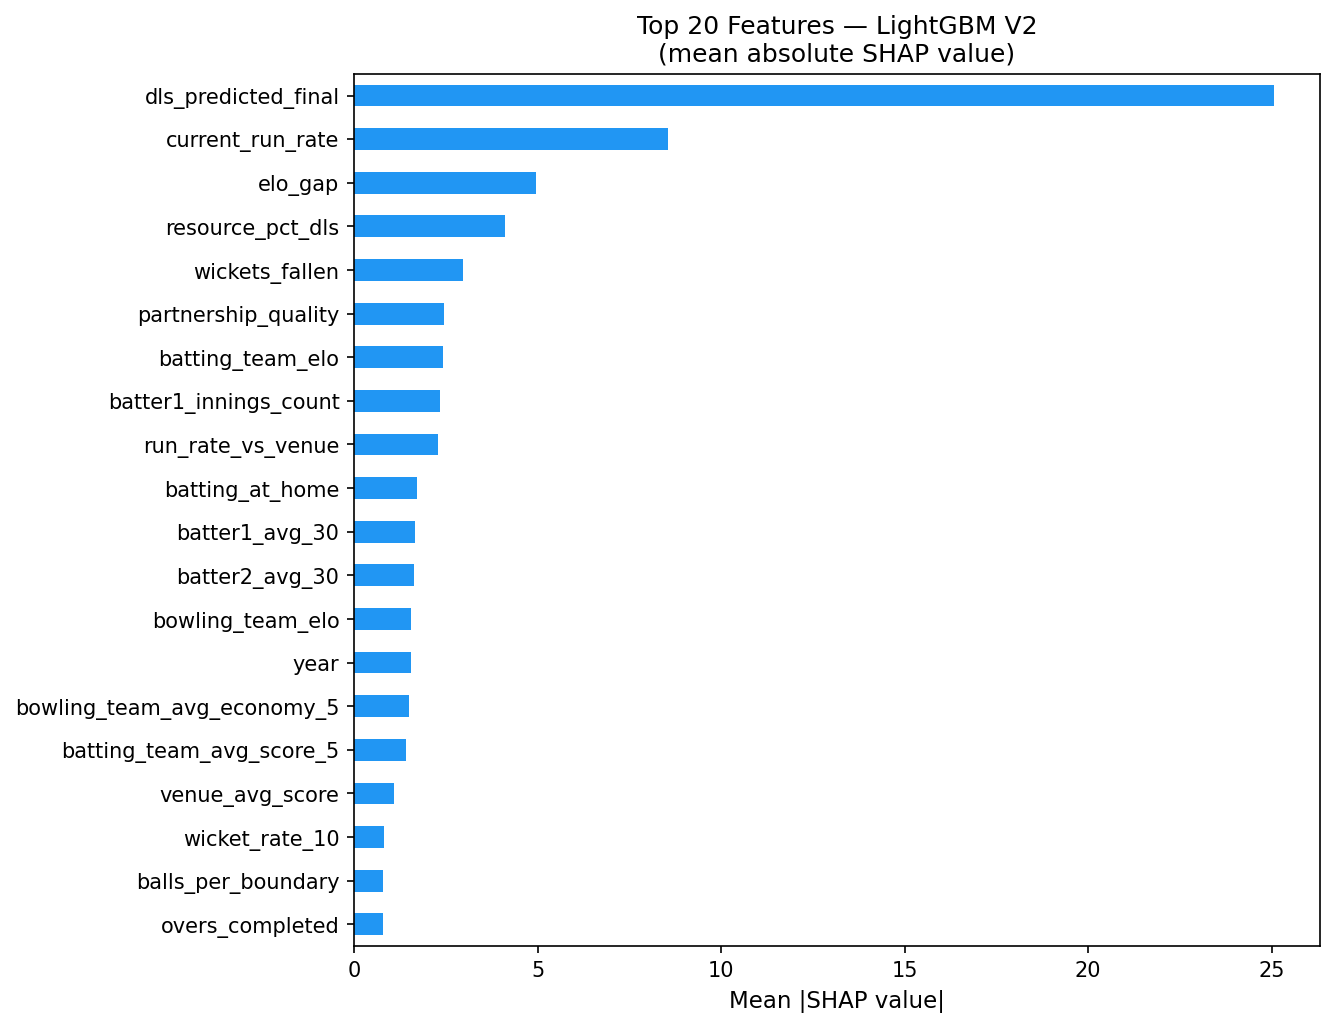
\includegraphics[width=0.97\columnwidth]{mens_odi_shap_bar_lgb_v2.png}
\caption{Mean absolute SHAP values (LightGBM, top 20 features). \texttt{dls\_predicted\_final} dominates ($\approx$25 run-units), confirming that ML models use the DLS projection as a primary baseline. \texttt{current\_run\_rate} is second ($\approx$8.5 units), capturing real-time momentum. Player features (\texttt{partnership\_quality}, \texttt{batter1\_avg\_30}) and Elo appear in the mid-range.}
\label{fig:shap_bar_lgb}
\end{figure}

\begin{figure}[htbp]
\centering
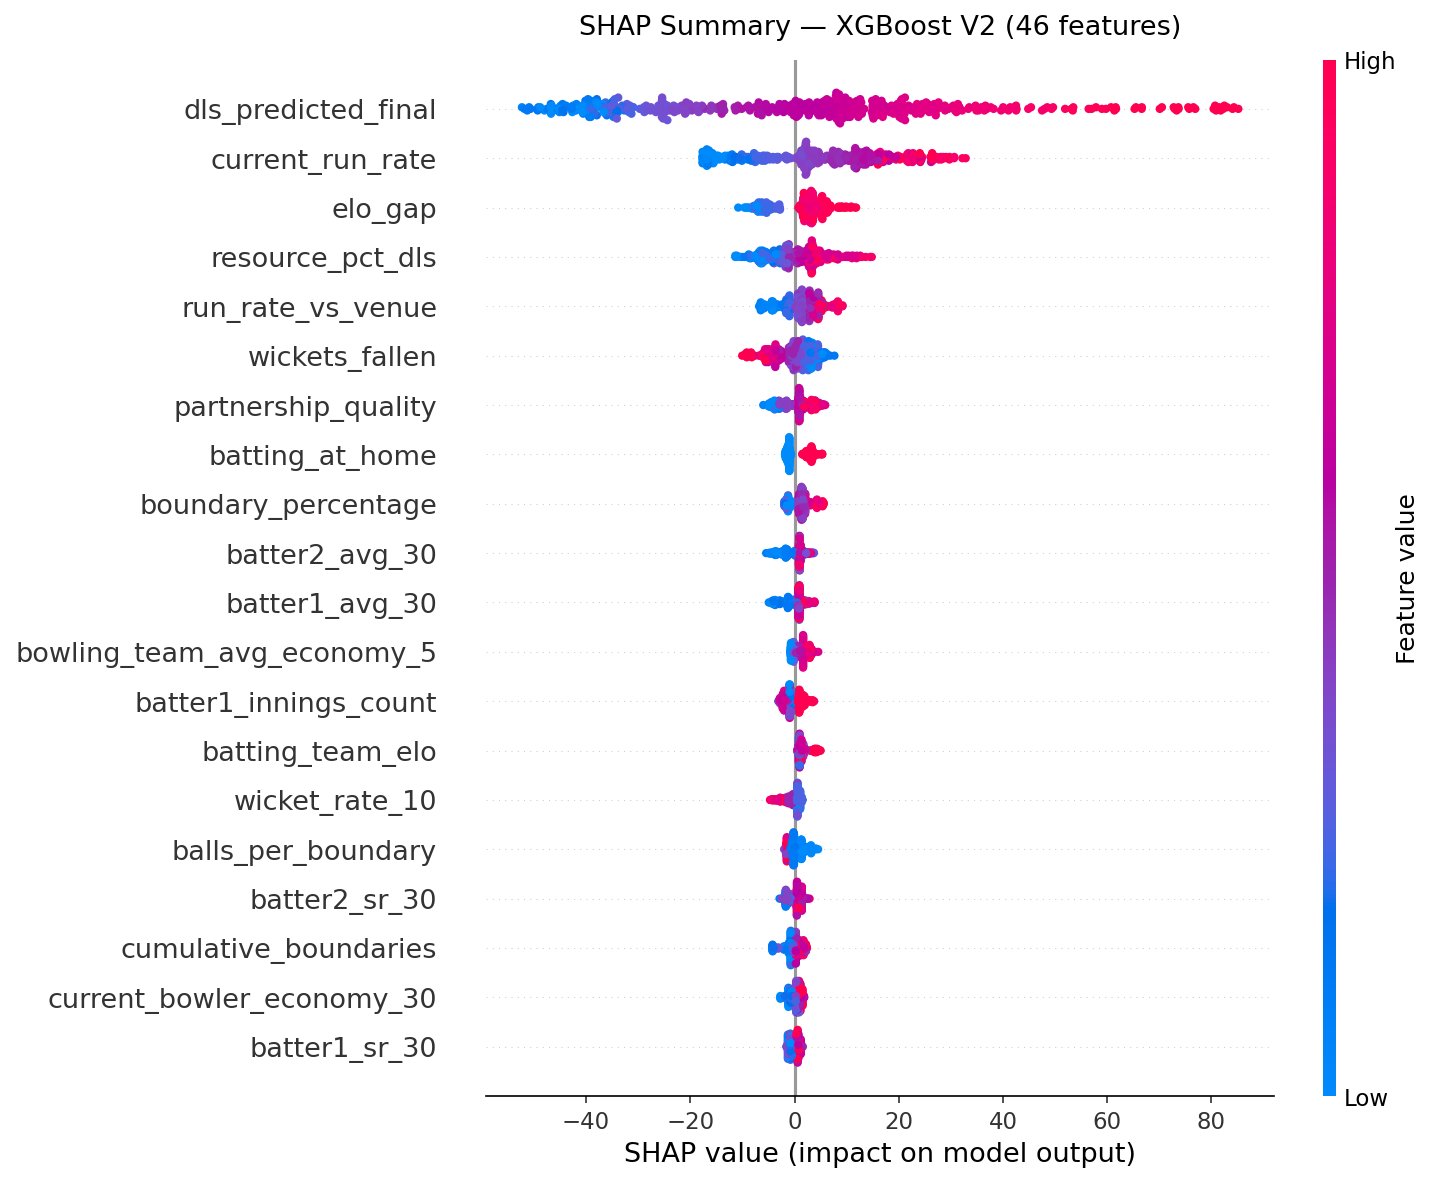
\includegraphics[width=0.97\columnwidth]{mens_odi_shap_summary_xgboost_v2.png}
\caption{SHAP beeswarm plot (XGBoost, 46 features). Each point = one test snapshot; horizontal position = SHAP value (impact on prediction); colour = feature value (red = high, blue = low). \texttt{dls\_predicted\_final} (top) shows clear positive relationship. \texttt{wickets\_fallen} shows strong negative effect consistent with cricket intuition.}
\label{fig:shap_summary}
\end{figure}

SHAP analysis (Figures~\ref{fig:shap_bar_lgb}--\ref{fig:shap_summary}) addresses \textbf{RQ3} and \textbf{RQ4}. The dominant importance of \texttt{dls\_predicted\_final} ($\approx$25 SHAP units) confirms the residual-learning framework: ML models learn corrections on top of the DLS projection, not an entirely independent prediction. The second-most important feature, \texttt{current\_run\_rate} ($\approx$8.5 units), captures real-time scoring momentum---information entirely absent from the DLS two-variable framework. \texttt{elo\_gap} and \texttt{resource\_pct\_dls} follow, reflecting team strength differentials and innings stage. Player features (\texttt{partnership\_quality}, \texttt{batter1\_avg\_30}) and Elo ratings contribute in the mid-range, while venue and momentum features form a long lower tier that is individually modest but collectively important as confirmed by ablation. The beeswarm plot (Figure~\ref{fig:shap_summary}) shows that high values of \texttt{dls\_predicted\_final} and \texttt{current\_run\_rate} push predictions upward, while high \texttt{wickets\_fallen} pushes them downward---all consistent with cricket domain knowledge, providing the interpretability required for practical adoption.

\begin{figure}[htbp]
\centering
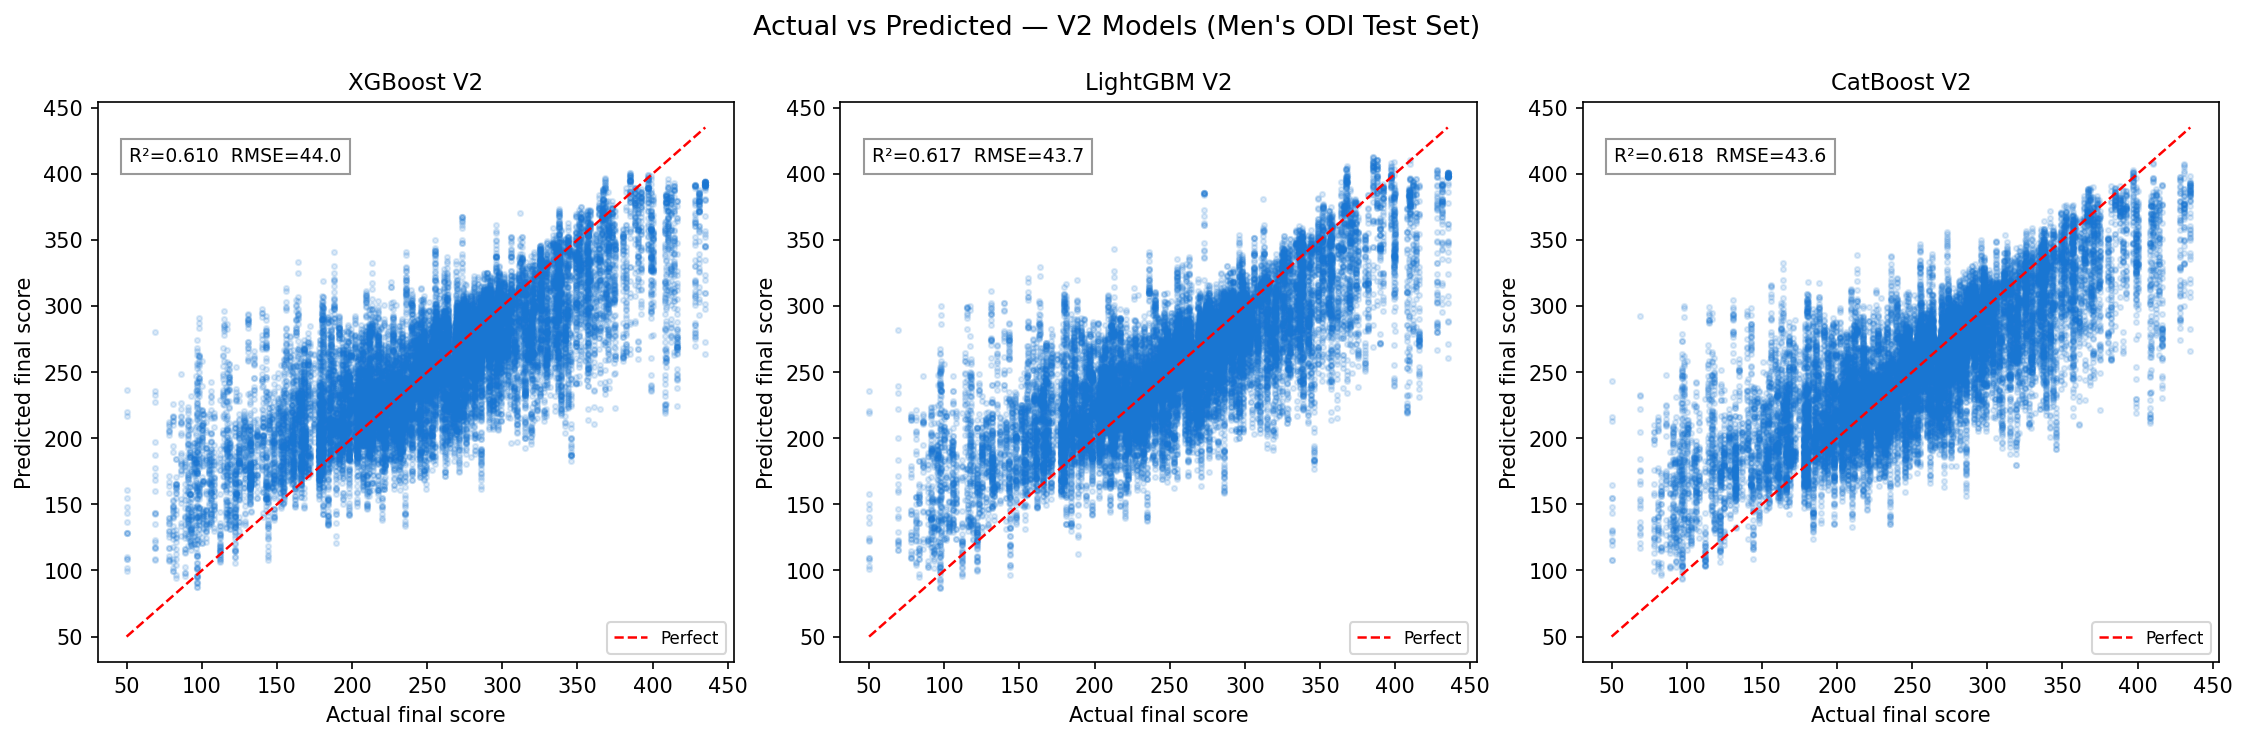
\includegraphics[width=0.97\columnwidth]{mens_odi_actual_vs_predicted_v2.png}
\caption{Actual vs.\ predicted first-innings scores for XGBoost, LightGBM, CatBoost (left to right) on the test set. All three produce tight scatter around the diagonal with $R^2\approx0.62$ and negligible systematic bias.}
\label{fig:actual_pred}
\end{figure}

\begin{figure}[htbp]
\centering
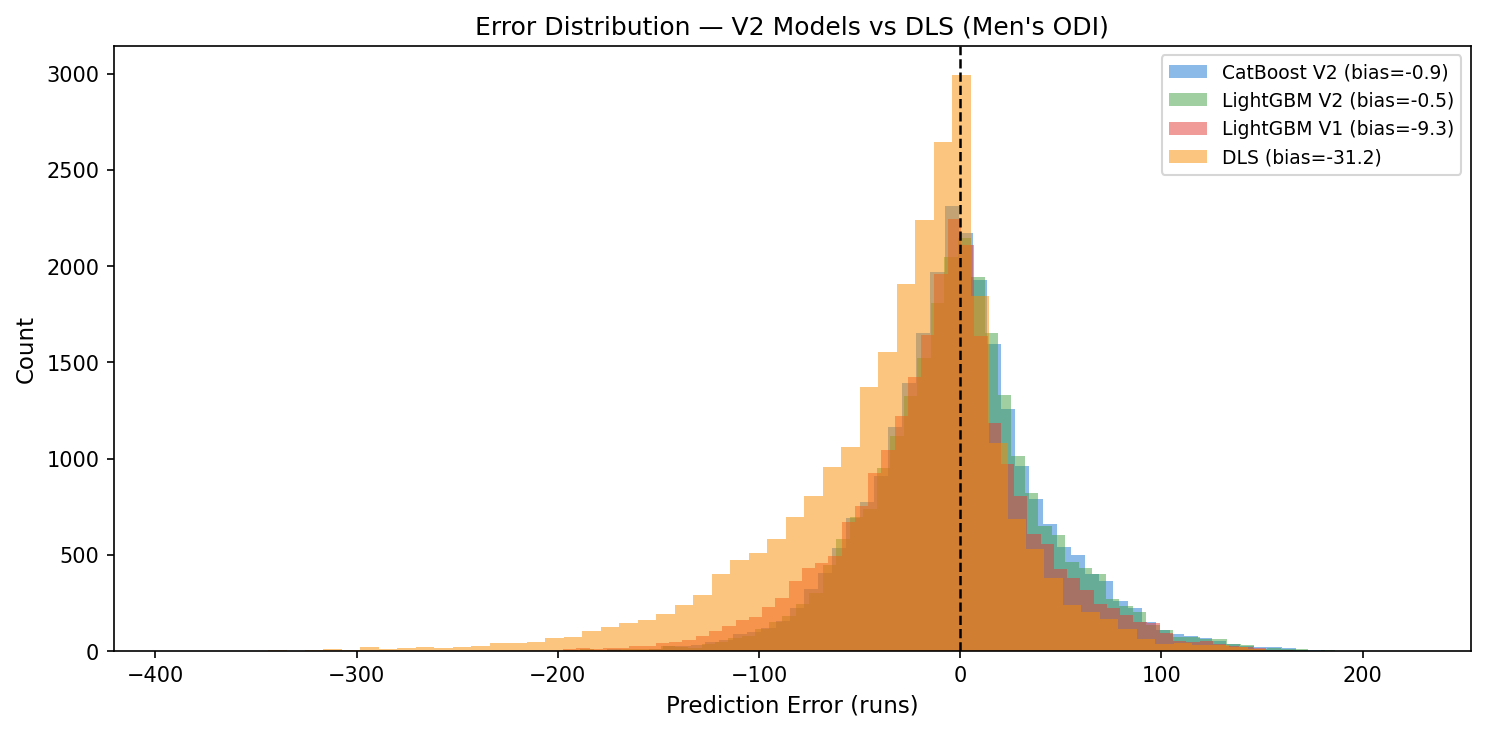
\includegraphics[width=0.97\columnwidth]{mens_odi_error_dist_v2.png}
\caption{Prediction error distributions (actual minus predicted) on the first-innings test set. ML models are tightly centred near zero. DLS exhibits a heavy left tail (mean bias $-31.2$ runs), reflecting systematic over-prediction---most severe in early overs.}
\label{fig:error_dist}
\end{figure}

Figure~\ref{fig:actual_pred} shows actual versus predicted scatter plots for all three GBMs, with tight clustering around the diagonal ($R^2 \approx 0.62$) and no obvious nonlinear bias patterns. Figure~\ref{fig:error_dist} presents error distributions: ML models produce distributions tightly centred near zero (CatBoost bias $-0.9$ runs, LightGBM bias $-0.5$ runs), while DLS exhibits a pronounced heavy left tail with mean bias $-31.2$ runs. This DLS systematic over-prediction is most severe in early overs where the resource function extrapolates from minimal information.

% ============================================================
\section{Economic Implications}
\label{sec:economics}
% ============================================================

\subsection{Motivating Cases}

Three historical incidents illustrate that target-setting accuracy has direct economic and competitive consequences, not merely statistical ones.

\textbf{1992 World Cup Semi-final (South Africa vs.\ England):} This pre-DLS incident---using the ``most productive overs'' rule---required South Africa to score an impossible \textbf{21 off 1 ball} after a 12-minute rain delay, eliminating them from the tournament's final four. Under retrospective DLS calculation, South Africa would have needed only 5 runs from the final delivery---a routine task. This match directly motivated DLS's development and first international use in January 1997 \citep{cricinfo_sa1992}.

\textbf{2003 World Cup (South Africa vs.\ Sri Lanka, Durban):} South Africa, pursuing 269, were at 229/6 off 45 overs when rain arrived. A critical \textbf{miscommunication of the DLS par score} led batsman Mark Boucher to believe 229 was the winning score; he defensively blocked the last ball. In fact, 229 was the tie score: they needed 230 to advance. South Africa were eliminated---the first host nation to exit a Cricket World Cup at the group stage \citep{wisden2003}. The economic consequence: failure to reach the knockout stages cost substantial prize money and long-term sponsorship visibility.

\textbf{2022 T20 World Cup (India vs.\ Bangladesh, Adelaide):} Bangladesh were 66/0 off 6.2 overs---well ahead of DLS par---when rain halted play. The revised target of 151 off 16 overs (rather than the original 184 off 20) was widely criticised as too generous to India. Bangladesh lost by 5 runs, with direct implications for Super 12 qualification. The ICC T20 World Cup 2024 prize pool reached a record US\$11.25 million \citep{icc_t20_2024prizes}; similar financial stakes applied in 2022.

These cases establish that DLS errors or near-errors have occurred at the highest stakes of world cricket. The broader context is amplified by cricket's vast betting ecosystem: cricket betting in India alone is estimated at \textbf{US\$100--150 billion annually} (combined legal and illegal markets), making cricket the world's second-largest sports betting market after European football. Incorrectly set rain targets shift match odds significantly, creating information asymmetries between bettors with access to more accurate models and those relying solely on official DLS targets.

\subsection{Economic Framework}

We adopt two complementary frameworks from welfare economics and decision theory.

\textbf{Gini coefficient analysis \citep{Gini1912}:} The Gini coefficient $G \in [0,1]$ is applied to the distribution of prediction RMSE across ICC member nations. $G=0$ means all nations bear equal prediction error burden; $G=1$ means one nation bears all error. We plot Lorenz curves to visualise the distribution of DLS vs.\ ML error burden across national boards spanning extreme revenue ranges (BCCI: \$1.7 billion/year; Associate members: under \$2 million).

\textbf{Expected Value of Information \citep{Howard1966}:} The economic value of prediction accuracy in an interrupted match is:
\begin{equation}
\text{EVI} = P(\text{outcome changes} \mid \Delta T) \times \Delta\text{Prize}
\end{equation}
where $\Delta T = |T_\text{ML} - T_\text{DLS}|$ is the target revision magnitude and $\Delta\text{Prize}$ is the prize differential between advancing and exiting at the given tournament stage. We model $P(\text{outcome changes} \mid \Delta T)$ using an exponential model calibrated to the historical ODI median winning margin of 18 runs:
\begin{equation}
P(\text{outcome changes} \mid \Delta T) = 1 - e^{-\Delta T / 18}
\end{equation}
This yields a conservative lower bound: at the observed mean $|\Delta T| = 42.7$ runs, $P(\text{change}) \approx 90.7\%$.

\subsection{Fairness Equity Analysis Across ICC Member Nations}

\begin{table*}[htbp]
\centering
\caption{Per-nation first-innings RMSE by ICC economic tier. Board revenue estimates based on publicly reported ICC financial distributions (2022--2024). DLS advantage = DLS RMSE $-$ ML RMSE (runs saved by switching to ML).}
\label{tab:econ_fairness}
\small
\begin{tabular}{llrrrrr}
\toprule
\textbf{Nation} & \textbf{Tier} & \textbf{Rev.\ (USD M)} & \textbf{DLS RMSE} & \textbf{ML RMSE} & \textbf{Advantage} & \textbf{Rel.\ (\%)} \\
\midrule
India           & 1 (Major) & 1170 & 66.78 & 43.22 & 23.56 & 35.3 \\
Australia       & 1 (Major) &  180 & 67.29 & 46.36 & 20.93 & 31.1 \\
England         & 1 (Major) &  200 & 73.88 & 46.20 & 27.68 & 37.5 \\
\midrule
New Zealand     & 2 (Mid)   &   35 & 68.89 & 43.44 & 25.45 & 36.9 \\
South Africa    & 2 (Mid)   &   40 & 79.11 & 56.91 & 22.20 & 28.1 \\
Sri Lanka       & 2 (Mid)   &   25 & 54.45 & 36.98 & 17.47 & 32.1 \\
\midrule
Bangladesh      & 3 (Small) &   15 & 55.90 & 37.07 & 18.83 & 33.7 \\
Ireland         & 3 (Small) &    7 & 57.55 & 37.57 & 19.98 & 34.7 \\
\midrule
Scotland        & 4 (Assoc) &    2 & 69.81 & 44.19 & 25.62 & 36.7 \\
UAE             & 4 (Assoc) &    2 & 51.33 & 43.78 &  7.55 & 14.7 \\
\midrule
\multicolumn{7}{l}{\small Gini DLS = 0.076; Gini ML = 0.067. Spearman($\rho$, revenue, DLS RMSE) $= 0.44$, $p=0.21$. Kruskal-Wallis $H=1.76$, $p=0.62$.} \\
\bottomrule
\end{tabular}
\end{table*}

Table~\ref{tab:econ_fairness} reports per-nation prediction RMSE. The Gini coefficient of DLS RMSE across nations is $G_\text{DLS} = 0.076$; for the best ML model, $G_\text{ML} = 0.067$---a 12\% reduction. Both values are close to zero, indicating that DLS prediction error is broadly equitable across nations: no single tier bears a massively disproportionate error burden. The Kruskal-Wallis test finds no statistically significant difference in DLS RMSE across tiers ($H=1.76$, $p=0.62$), and Spearman's rank correlation between board revenue and DLS RMSE is non-significant ($\rho=0.44$, $p=0.21$). This uniformity of DLS error is partly by design: the universal resource table does not adapt to team-specific playing styles.

The ML advantage is largest in absolute terms for England ($+27.7$ runs) and India ($+23.6$ runs), which feature more extreme scoring environments. The relative improvement is broadly consistent across tiers (28--37\%), except for UAE (14.7\%) where sparse test samples suppress variance estimates. Critically, while DLS errors are equitably distributed by RMSE, their economic impact differs drastically across boards: a 20-run DLS error in a group-stage match carries far more consequence for Ireland (board revenue $\approx$\$7M/year, every ICC prize crucial to long-term viability) than for India (board revenue $\approx$\$1.17~billion/year \citep{sportsmint2024bcci}). The broader ICC revenue distribution reveals extreme inequality: BCCI receives approximately 38.5\% of ICC annual net earnings ($\approx$\$230~million/year), while all remaining Full Members share the remaining $\sim$49\% \citep{espncricinfo_bcci_share}.

\begin{figure*}[htbp]
\centering
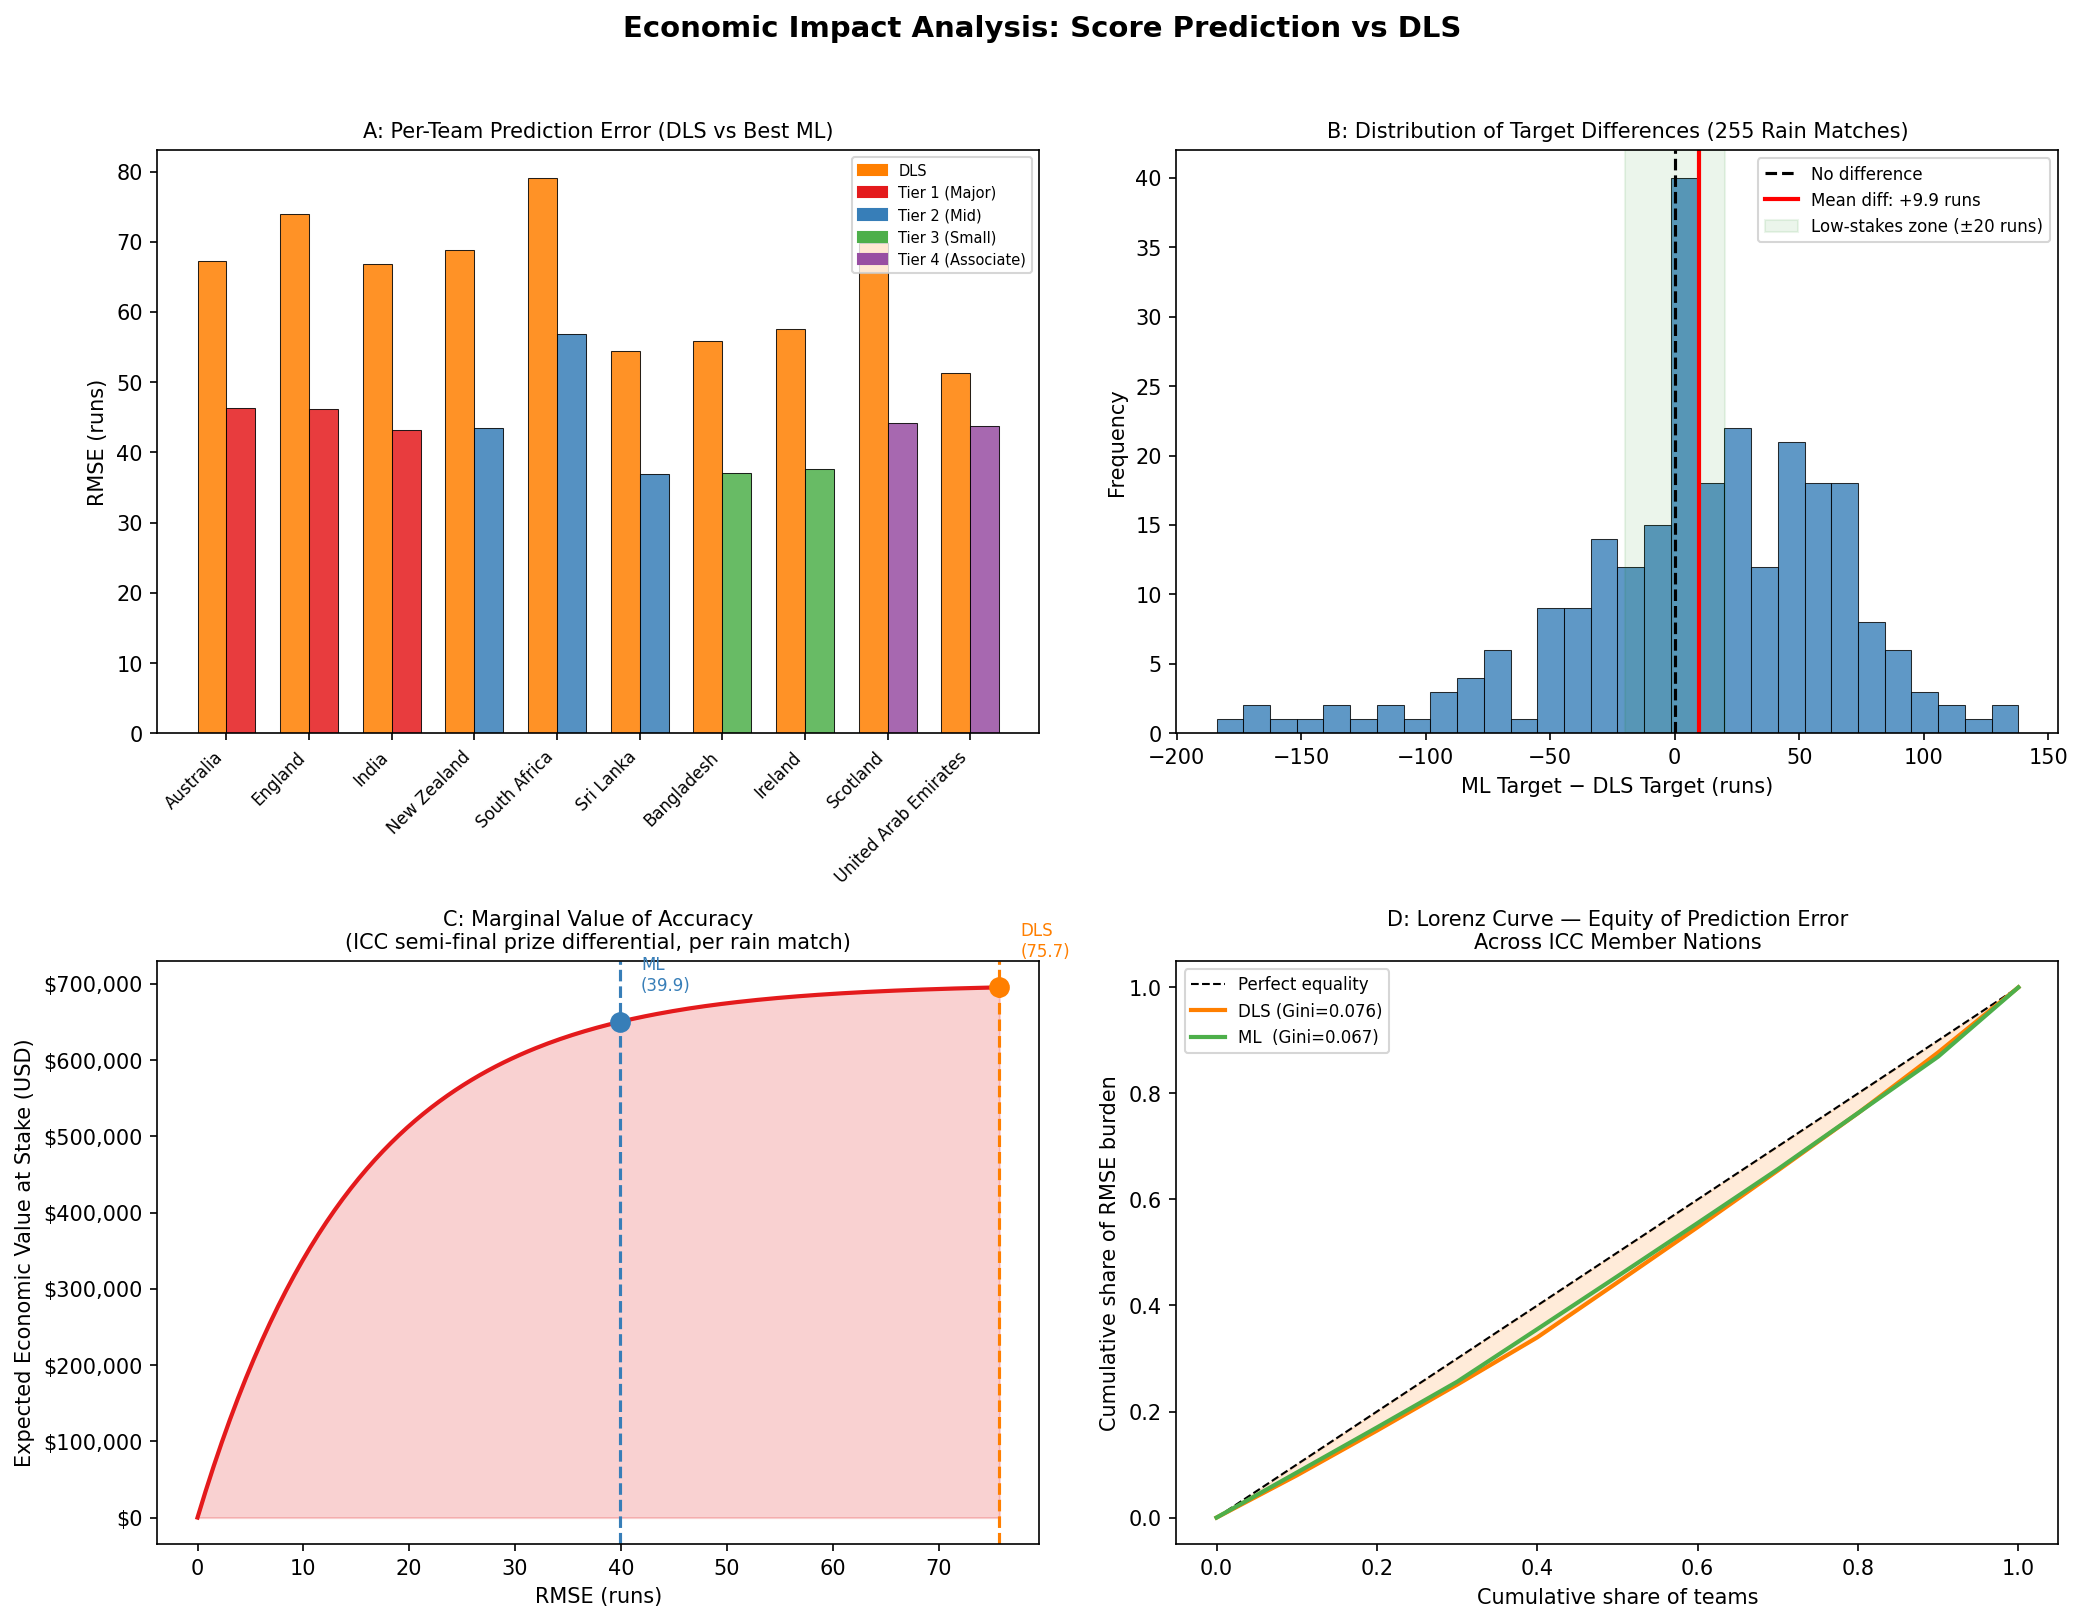
\includegraphics[width=0.97\textwidth]{economic_fairness.png}
\caption{Economic impact analysis. \textbf{(A)} Per-nation DLS vs.\ ML RMSE, colour-coded by economic tier. \textbf{(B)} Distribution of ML $-$ DLS target revisions across 255 historical rain-affected matches; mean revision $+9.9$ runs ($t=2.88$, $p=0.004$). \textbf{(C)} Marginal Value of Accuracy curve for an ICC semi-final match. \textbf{(D)} Lorenz curves for DLS ($G=0.076$) and ML ($G=0.067$) prediction error across ICC nations.}
\label{fig:economic_fairness}
\end{figure*}

\subsection{Target-Setting Bias in Rain-Affected Matches}

The 255 historical D/L-affected matches provide direct evidence of systematic target-setting differences between DLS and the ML revised target engine (Table~\ref{tab:revised_targets}). The ML engine sets targets $+9.9$ runs higher than DLS on average, a difference statistically significant at $p=0.004$ (one-sample $t$-test against zero, $t=2.88$). In 64.7\% of the 255 matches, the ML engine revises the target upward relative to DLS. This directional asymmetry has an economic interpretation: DLS systematically advantages the batting (chasing) team by setting lower targets, potentially benefiting teams with superior chasing records or those playing in run-friendly conditions.

In 66.7\% of rain-affected matches, the absolute target difference exceeds 20 runs---a magnitude typically associated with a competitive ODI victory margin. The ML engine's substantially lower standard deviation (42.4 vs.\ 63.0 runs) reflects its regression-to-the-mean behaviour: DLS's wider distribution reflects its design to handle extreme scenarios (e.g., interruption at over 2), where the resource table extrapolation can produce very high or very low targets. The ML's narrower distribution reduces the risk of economically perverse outcomes, such as a 2nd-over interruption resulting in a target of 280+ runs.

\subsection{Economic Value Framework}

\begin{table}[htbp]
\centering
\caption{Expected economic value at stake per interrupted match at ICC Men's ODI World Cup 2023 prize schedule \citep{ICC2023prizes}. EVI $= P(\text{change}) \times \Delta\text{Prize}$; $P(\text{change})=0.907$ at mean $|\Delta T|=42.7$ runs.}
\label{tab:econ_value}
\small
\begin{tabular}{lrrr}
\toprule
\textbf{Stage} & $\Delta$\textbf{Prize} & $P$\textbf{(change)} & \textbf{EV/Match} \\
\midrule
WC Final (winner) & \$2{,}000{,}000 & 0.907 & \$1{,}813{,}433 \\
WC Semi-final     & \$1{,}400{,}000 & 0.907 & \$1{,}269{,}403 \\
WC Group Stage    & \$1{,}500{,}000 & 0.907 & \$1{,}360{,}075 \\
\bottomrule
\end{tabular}
\end{table}

Table~\ref{tab:econ_value} presents the decision-theoretic expected value at stake per interrupted match. At the mean absolute target difference of 42.7 runs, $P(\text{outcome changes}) = 1 - e^{-42.7/18} \approx 0.907$, meaning there is a 90.7\% probability that an average rain-match target revision is large enough to potentially change the match outcome. At the ICC World Cup Final stage, an incorrectly set target places an expected \$1.81 million of prize money at risk. Even at the group-stage level, expected prize exposure per match is \$1.36 million---economically significant for any board. Across a typical 45-48 match tournament, even two or three rain interruptions represent multiple millions of dollars in potentially misallocated prize money.

Moving from the DLS second-innings RMSE (75.74) to the ML RMSE (39.92) reduces the expected value-at-stake by approximately \$44,987 per interrupted semi-final---a direct economic benefit of the improved model. The diminishing-returns shape of the Marginal Value of Accuracy (MVA) curve (Figure~\ref{fig:economic_fairness}C) indicates that the largest marginal economic gains come from reducing error in the 20--60 run RMSE range, precisely where the DLS-to-ML improvement falls.

\subsection{Policy Implications}

The economic analysis motivates three actionable policy recommendations.

\textbf{(1) ML-augmented target review:} Given the 52.9\% winner-disagreement rate between ML and DLS and the statistically significant DLS downward bias ($+9.9$ runs, $p=0.004$), the ICC could consider ML predictions as an advisory tool for match referees when the DLS target appears anomalous. This does not require replacing DLS---which has regulatory legitimacy and wide acceptance---but providing an independent data-driven estimate for verification.

\textbf{(2) Uncertainty disclosure:} The conformal prediction intervals (mean width 129 runs at 90\% nominal coverage) provide a distribution-free uncertainty quantification for any score projection. Publishing these intervals alongside official DLS targets would give batting teams and audiences an honest quantification of the precision with which any target is set, particularly in early-innings interruptions where uncertainty is highest.

\textbf{(3) Associate nation equity:} Although the Gini analysis finds DLS error is broadly equitable across tiers, the absolute RMSE remains high (51--70 across nations). For Associate nations (UAE, Scotland, Netherlands) with smaller player pools and less consistent scoring patterns, targeted ball-by-ball data collection at Associate-level ICC events would enable personalised models with better generalisation, directly improving competitive fairness.

% ============================================================
\section{Conclusion}
\label{sec:conclusion}
% ============================================================

\subsection{Summary of Findings}

This paper has presented a comprehensive empirical investigation of machine learning as an alternative to the DLS method in limited-overs cricket. Key findings by research question:

\textbf{RQ1 -- ML vs.\ DLS first innings:} CatBoost achieves RMSE~43.57, $R^2=0.618$---a 33\% RMSE reduction over DLS (RMSE~65.03, $R^2=0.150$). All three DM tests reject equal predictive accuracy at $p < 0.001$ (Bonferroni-corrected). DLS performs catastrophically in Early overs ($R^2 = -1.008$, RMSE~105.0), worse than predicting the mean---a consequence of resource-fraction extrapolation from minimal information. ML improves 42\% in Early overs, 24\% in Middle overs, and marginally in Death overs (all three phases, no exception).

\textbf{RQ2 -- Phase analysis:} ML outperforms DLS in all three innings phases. In Death overs, all systems converge to RMSE~15--16 as the outcome is nearly determined. In Early overs, the performance gap is largest (DLS $R^2 = -1.008$ vs.\ ML $R^2 \approx 0.32$). The 95\% bootstrap CI for RMSE difference is $[-23.94, -18.72]$ runs, entirely below zero.

\textbf{RQ3 -- Feature importance:} SHAP analysis identifies DLS-derived features (\texttt{dls\_predicted\_final}, \texttt{resource\_pct\_dls}) and \texttt{current\_run\_rate} as the top contributors. Player statistics (+3.4\% RMSE ablation impact) and DLS features (+3.0\%) are the most critical groups, while venue, Elo, and momentum features are individually modest but collectively important.

\textbf{RQ4 -- Explainability:} SHAP values are consistent with cricket domain knowledge throughout: high DLS projections push ML predictions upward; high wickets fallen push them downward; high current run rate increases projected totals. LIME analysis provides instance-level explanations suitable for broadcast commentary contexts.

\textbf{RQ5 -- Conformal prediction:} MAPIE split conformal prediction at $\alpha=0.10$ achieves 86.6\% empirical coverage (vs.\ 90\% nominal) with mean interval width 129 runs. The 3.4-percentage-point coverage gap is attributable to temporal non-exchangeability, not model miscalibration. The MCS at $\alpha=0.10$ contains \{CatBoost, LightGBM\}; XGBoost is eliminated.

\textbf{RQ6 -- Extended architectures:} The stacking meta-learner achieves RMSE~43.39 (best overall). Monotonic XGBoost costs only $+0.14$ RMSE for guaranteed physical validity. OLS on 46 features (RMSE~43.34) matches individual GBMs, establishing that the feature engineering pipeline---not model architecture---is the primary driver of improvement. The V3 55-feature extension provides no meaningful gain over V2 ($|\Delta\text{RMSE}| < 0.3$).

\textbf{RQ7 -- Temporal stability:} Walk-forward CV ($K=5$) yields LightGBM RMSE~$40.96 \pm 2.35$ runs across eras spanning 2016--2026, with ML--DLS gap stable at $-20.44 \pm 2.79$ runs in every fold. Concept drift analysis shows ML RMSE improving over time (negative Pearson $r$) while DLS degrades (positive $r$), with a DLS RMSE range three times larger than ML.

\textbf{RQ8 -- Economic implications:} On 255 D/L matches, ML sets targets $+9.9$ runs higher than DLS ($t=2.88$, $p=0.004$), with 52.9\% winner disagreement. Gini analysis shows DLS error is broadly equitable ($G=0.076$) but ML is marginally more equitable ($G=0.067$). At the ICC World Cup semi-final stage, DLS-level accuracy places an expected \$1.27 million of prize money at risk per interrupted match under the decision-theoretic EVI framework.

\subsection{Limitations}

\begin{enumerate}[leftmargin=1.2em]
\item \textbf{Censoring in second innings:} The 49.2\% right-censoring rate forces training on uncensored (losing) innings only. The 8-run selection bias is documented but not corrected; a Tobit treatment is left for future work.
\item \textbf{Reduced-overs extrapolation:} The revised target engine extrapolates beyond the training distribution when predicting scores for severely curtailed innings (e.g., match reduced to 10 overs from over 8).
\item \textbf{Men's ODI focus only:} Women's cricket and T20 formats have different scoring dynamics; the full pipeline would require separate fitting for each format.
\item \textbf{No ball-by-ball sequence modelling:} Features are computed at over boundaries. A BiLSTM or Transformer encoder on ball-by-ball sequences could capture intra-over momentum shifts that over-boundary snapshots necessarily aggregate.
\end{enumerate}

\subsection{Future Work}

Key extensions include: (1) Tobit regression for right-censored second innings to recover unbiased regression coefficients under the censoring mechanism; (2) BiLSTM/Transformer sequence models on ball-by-ball delivery sequences using the PyTorch MPS backend on Apple Silicon; (3) reduced-overs-aware training by augmenting the second-innings dataset with deliberately curtailed innings; (4) extension to Women's ODI and T20I formats; (5) a win-probability classifier setting ML targets such that $P(\text{win} | T^*) = 0.5$, operationalising the DLS fairness principle directly; (6) real-time deployment as a FastAPI microservice with SHAP attribution for broadcast integration; (7) player matchup features exploiting batter-bowler dismissal rates from ball-by-ball records using LASSO-regularised mixed-effects models.

\subsection{Concluding Remarks}

The DLS method has served cricket admirably for over two decades, offering transparency and a principled resource-accounting framework. This paper demonstrates that machine learning models can substantially improve upon DLS's predictive accuracy across both innings and all match phases, that these improvements are statistically significant at conventional levels with strong effect sizes, and that the key features driving ML performance align with cricket domain knowledge revealed through SHAP analysis---providing the interpretability required for practical adoption.

A central finding is that the improvement over DLS is not attributable to complex model architectures: even ordinary least squares regression on the 46 engineered features achieves comparable accuracy to state-of-the-art gradient boosting. This establishes that the \textbf{feature engineering pipeline}---specifically the temporally safe construction of Elo ratings, rolling player statistics, and historical venue profiles---is the primary scientific contribution. As cricket continues to evolve with T10 leagues, franchise cricket, and changing pitch preparation practices altering scoring distributions, data-driven approaches offer the adaptability to track these changes automatically through periodic retraining. The future of cricket target-setting likely lies in hybrid systems combining the domain-knowledge foundation of DLS with the contextual flexibility of machine learning, guided by the statistical rigour demonstrated in this work.

% ============================================================
% Bibliography
% ============================================================
\bibliographystyle{apalike}

\begin{thebibliography}{99}

\bibitem[Akiba et~al., 2019]{akiba2019optuna}
Akiba, T., Sano, S., Yanase, T., Ohta, T., and Koyama, M. (2019).
\newblock Optuna: A next-generation hyperparameter optimization framework.
\newblock In \emph{Proc.\ 25th ACM SIGKDD}, pp.~2623--2631.

\bibitem[Baboota and Kaur, 2019]{baboota2019predictive}
Baboota, R. and Kaur, H. (2019).
\newblock Predictive analysis and modelling football results using machine learning for the English Premier League.
\newblock \emph{International Journal of Forecasting}, 35(2):741--755.

\bibitem[Bhattacharya et~al., 2011]{bhattacharya2011revised}
Bhattacharya, R., Gill, P.~S., and Swartz, T.~B. (2011).
\newblock A revised Duckworth-Lewis method for Twenty20 cricket.
\newblock \emph{Journal of the Operational Research Society}, 62(12):2187--2193.

\bibitem[Breiman, 2001]{breiman2001random}
Breiman, L. (2001).
\newblock Random forests.
\newblock \emph{Machine Learning}, 45(1):5--32.

\bibitem[Bunker and Thabtah, 2019]{bunker2019machine}
Bunker, R.~P. and Thabtah, F. (2019).
\newblock A machine learning framework for sport result prediction.
\newblock \emph{Applied Computing and Informatics}, 15(1):27--33.

\bibitem[Carter and Guthrie, 2005]{carter2005model}
Carter, M. and Guthrie, G. (2005).
\newblock A model for cricket run rates.
\newblock \emph{Teaching Statistics}, 27(3):84--87.

\bibitem[Chen and Guestrin, 2016]{chen2016xgboost}
Chen, T. and Guestrin, C. (2016).
\newblock {XGBoost}: A scalable tree boosting system.
\newblock In \emph{Proc.\ 22nd ACM SIGKDD}, pp.~785--794.

\bibitem[Cohen, 1988]{Cohen1988}
Cohen, J. (1988).
\newblock \emph{Statistical Power Analysis for the Behavioral Sciences} (2nd ed.).
\newblock Lawrence Erlbaum Associates.

\bibitem[Cricsheet, 2024]{cricsheet}
Cricsheet (2024).
\newblock Cricket match data. \url{https://cricsheet.org/}.

\bibitem[Davis et~al., 2015]{davis2015investigating}
Davis, J., Perera, H., and Swartz, T.~B. (2015).
\newblock Investigating the effect of the toss in Twenty20 cricket.
\newblock \emph{Journal of Quantitative Analysis in Sports}, 11(2):75--85.

\bibitem[Deep et~al., 2016]{deep2016learning}
Deep, S., Singh, B., and Kumar, V. (2016).
\newblock Learning with recurrent neural networks for cricket match prediction.
\newblock \emph{International Journal of Computer Applications}, 145(9):1--6.

\bibitem[Diebold and Mariano, 1995]{diebold1995comparing}
Diebold, F.~X. and Mariano, R.~S. (1995).
\newblock Comparing predictive accuracy.
\newblock \emph{Journal of Business \& Economic Statistics}, 13(3):253--263.

\bibitem[Duckworth and Lewis, 1998]{duckworth1998}
Duckworth, F.~C. and Lewis, A.~J. (1998).
\newblock A fair method for resetting the target in interrupted one-day cricket matches.
\newblock \emph{Journal of the Operational Research Society}, 49(3):220--227.

\bibitem[ESPNcricinfo, 1992]{cricinfo_sa1992}
ESPNcricinfo (2020).
\newblock South Africa end up on the receiving end of a rain-rule farce.
\newblock \url{https://www.espncricinfo.com/story/south-africa-end-up-on-the-receiving-end-of-a-rain-rule-farce-in-the-world-cup-508066}

\bibitem[ESPNcricinfo, 2024]{espncricinfo_bcci_share}
ESPNcricinfo (2024).
\newblock BCCI set to get nearly 40\% of ICC's annual net earnings.
\newblock \url{https://www.espncricinfo.com/story/bcci-set-to-get-nearly-40-of-icc-s-annual-net-earnings-1387167}

\bibitem[Gini, 1912]{Gini1912}
Gini, C. (1912).
\newblock Variabilit\`a e mutabilit\`a.
\newblock \emph{Memorie di Metodologica Statistica}. Libreria Eredi Virgilio Veschi.

\bibitem[Hansen et~al., 2011]{hansen2011model}
Hansen, P.~R., Lunde, A., and Nason, J.~M. (2011).
\newblock The model confidence set.
\newblock \emph{Econometrica}, 79(2):453--497.

\bibitem[Howard, 1966]{Howard1966}
Howard, R.~A. (1966).
\newblock Information value theory.
\newblock \emph{IEEE Transactions on Systems Science and Cybernetics}, 2(1):22--26.

\bibitem[Huang and Chang, 2010]{huang2010neural}
Huang, M.~L. and Chang, Y.~S. (2010).
\newblock A neural network approach to predict baseball game scores.
\newblock In \emph{Proc.\ ICSCPR}, pp.~34--39.

\bibitem[ICC, 2023a]{icc2023}
International Cricket Council (2023).
\newblock Global cricket strategy 2023--2031. Technical report, ICC.

\bibitem[ICC, 2023b]{ICC2023prizes}
International Cricket Council (2023).
\newblock ICC Men's Cricket World Cup 2023: Prize Money.
\newblock \url{https://www.espncricinfo.com/story/odi-world-cup-2023-winner-to-receive-usd-4-million-1399559}

\bibitem[ICC, 2024]{icc_t20_2024prizes}
International Cricket Council (2024).
\newblock Record prize money for ICC Men's T20 World Cup 2024.
\newblock \url{https://www.icc-cricket.com/tournaments/t20cricketworldcup/news/record-prize-money-declared-for-t20-world-cup-2024}

\bibitem[Jhanwar and Pudi, 2016]{jhanwar2016predicting}
Jhanwar, M.~G. and Pudi, V. (2016).
\newblock Predicting the outcome of ODI cricket matches: A team composition based approach.
\newblock In \emph{Proc.\ ECML-PKDD Workshop}, pp.~1--16.

\bibitem[Kampakis and Thomas, 2015]{kampakis2015using}
Kampakis, S. and Thomas, W. (2015).
\newblock Using machine learning to predict the outcome of English county twenty over cricket matches.
\newblock \emph{arXiv:1511.05837}.

\bibitem[Ke et~al., 2017]{ke2017lightgbm}
Ke, G. et~al. (2017).
\newblock {LightGBM}: A highly efficient gradient boosting decision tree.
\newblock In \emph{NeurIPS}, vol.~30, pp.~3146--3154.

\bibitem[Lundberg and Lee, 2017]{lundberg2017unified}
Lundberg, S.~M. and Lee, S.~I. (2017).
\newblock A unified approach to interpreting model predictions.
\newblock In \emph{NeurIPS}, vol.~30, pp.~4765--4774.

\bibitem[Lundberg et~al., 2020]{lundberg2020local}
Lundberg, S.~M. et~al. (2020).
\newblock From local explanations to global understanding with explainable AI for trees.
\newblock \emph{Nature Machine Intelligence}, 2(1):2522--5839.

\bibitem[McHale and Asif, 2011]{mchale2011modelling}
McHale, I.~G. and Asif, M. (2011).
\newblock A modified Duckworth-Lewis method for adjusting targets in interrupted limited overs cricket.
\newblock \emph{European Journal of Operational Research}, 225(2):353--362.

\bibitem[Newey and West, 1987]{newey1987simple}
Newey, W.~K. and West, K.~D. (1987).
\newblock A simple, positive semi-definite, heteroskedasticity and autocorrelation consistent covariance matrix.
\newblock \emph{Econometrica}, 55(3):703--708.

\bibitem[Passi and Pandey, 2018]{passi2018cricket}
Passi, K. and Pandey, N. (2018).
\newblock Predicting players' performance in ODI cricket using machine learning.
\newblock \emph{Journal of Computer Science \& Systems Biology}, 11(4):1--8.

\bibitem[Prokhorenkova et~al., 2018]{prokhorenkova2018catboost}
Prokhorenkova, L. et~al. (2018).
\newblock {CatBoost}: unbiased boosting with categorical features.
\newblock In \emph{NeurIPS}, vol.~31.

\bibitem[Ribeiro et~al., 2016]{ribeiro2016should}
Ribeiro, M.~T., Singh, S., and Guestrin, C. (2016).
\newblock ``{W}hy should {I} trust you?'': Explaining the predictions of any classifier.
\newblock In \emph{Proc.\ 22nd ACM SIGKDD}, pp.~1135--1144.

\bibitem[Sankaranarayanan et~al., 2014]{sankaranarayanan2014auto}
Sankaranarayanan, V.~V., Sattar, J., and Lakshmanan, L.~V. (2014).
\newblock Auto-play: A data mining approach to ODI cricket simulation and prediction.
\newblock In \emph{Proc.\ SIAM SDM}, pp.~1064--1072.

\bibitem[{SciPy}, 2024]{scipy}
{SciPy Developers} (2024).
\newblock {SciPy}: Open source scientific tools for {Python}. \url{https://www.scipy.org/}.

\bibitem[SportsMint, 2024]{sportsmint2024bcci}
SportsMint Media (2024).
\newblock BCCI posts INR 9741.7 Cr in FY 2023--24 revenue.
\newblock \url{https://sportsmintmedia.com/bcci-posts-inr-9741-7-cr-in-fy-2023-24-revenue-as-ipl-dominates-earnings-mix/}

\bibitem[Stern, 2016]{stern2016}
Stern, S.~E. (2016).
\newblock The Duckworth-Lewis-Stern method: Extending the DL methodology to deal with modern scoring rates.
\newblock \emph{Journal of the Operational Research Society}, 67(12):1469--1480.

\bibitem[Taquet et~al., 2022]{taquet2022mapie}
Taquet, V. et~al. (2022).
\newblock {MAPIE}: an open-source library for distribution-free uncertainty quantification.
\newblock \emph{arXiv:2207.12274}.

\bibitem[Tobin, 1958]{tobin1958estimation}
Tobin, J. (1958).
\newblock Estimation of relationships for limited dependent variables.
\newblock \emph{Econometrica}, 26(1):24--36.

\bibitem[Viswanadha and Sivalenka, 2017]{viswanadha2017dynamic}
Viswanadha, S. and Sivalenka, K. (2017).
\newblock Dynamic prediction of cricket match outcomes using Bayesian networks.
\newblock \emph{International Journal of Sports Science \& Coaching}, 12(3):345--355.

\bibitem[Wisden, 2003]{wisden2003}
Wisden (2023).
\newblock Dead bat, miscalculations: South Africa's tragicomic 2003 World Cup exit recreated.
\newblock \emph{Wisden Cricketers' Almanack}. \url{https://www.wisden.com/series/asia-cup-2023/cricket-news/dead-bat-miscalculations-tragicomic-south-africa-2003-world-cup-exit-recreated-afghanistan}

\bibitem[Wolpert, 1992]{Wolpert1992}
Wolpert, D.~H. (1992).
\newblock Stacked generalization.
\newblock \emph{Neural Networks}, 5(2):241--259.

\bibitem[Zia et~al., 2022]{zia2022player}
Zia, S., Liaqat, H.~B., Zia, H.~U., Kong, X., and Shamshad, S. (2022).
\newblock Player-aware resource compensation in interrupted cricket matches.
\newblock \emph{PeerJ Computer Science}, 8:e917.

\end{thebibliography}

% ============================================================
% Appendix
% ============================================================
\appendix

\section{Fitted DLS Resource Table}
\label{app:resource_table}

Table~\ref{tab:resource_full} presents the fitted DLS resource percentages for selected (overs remaining, wickets lost) combinations, derived from the nonlinear least-squares fit of Equation~\ref{eq:dls} to 3,086 Men's ODI matches. Values decline monotonically with both increasing overs consumed and increasing wickets lost, consistent with the DLS model's resource-depletion interpretation.

\begin{table}[htbp]
\centering
\caption{Fitted DLS resource table (\% resources remaining)}
\label{tab:resource_full}
\tiny
\begin{tabular}{rrrrrrrrrrr}
\toprule
\textbf{Overs} & \textbf{w=0} & \textbf{w=1} & \textbf{w=2} & \textbf{w=3} & \textbf{w=4} & \textbf{w=5} & \textbf{w=6} & \textbf{w=7} & \textbf{w=8} & \textbf{w=9} \\
\midrule
50 & 100.0 & -- & -- & -- & -- & -- & -- & -- & -- & -- \\
40 & 87.5 & 82.1 & 76.2 & 69.5 & 61.8 & 53.0 & 42.6 & 31.7 & 21.1 & 10.3 \\
30 & 71.9 & 66.2 & 60.1 & 53.4 & 46.1 & 38.2 & 29.6 & 21.0 & 13.3 & 6.1 \\
20 & 53.4 & 48.0 & 42.4 & 36.5 & 30.4 & 24.2 & 17.9 & 12.0 & 7.2 & 3.1 \\
10 & 31.6 & 27.4 & 23.2 & 19.1 & 15.2 & 11.6 & 8.1 & 5.2 & 2.9 & 1.2 \\
5  & 17.3 & 14.6 & 12.0 & 9.7 & 7.5 & 5.5 & 3.8 & 2.3 & 1.3 & 0.5 \\
0  & 0.0 & 0.0 & 0.0 & 0.0 & 0.0 & 0.0 & 0.0 & 0.0 & 0.0 & 0.0 \\
\bottomrule
\end{tabular}
\end{table}

\section{Best Model Hyperparameters}
\label{app:hyperparams}

Best hyperparameters selected from Optuna Bayesian optimisation (100 trials for XGBoost, 50 each for LightGBM and CatBoost) on the 46-feature V2 pipeline.

\begin{table}[htbp]
\centering
\caption{XGBoost best hyperparameters (100 Optuna trials)}
\label{tab:xgb_params}
\small
\begin{tabular}{lr}
\toprule
\textbf{Parameter} & \textbf{Value} \\
\midrule
n\_estimators      & 425 \\
max\_depth         & 4 \\
learning\_rate     & 0.10079 \\
subsample          & 0.8032 \\
colsample\_bytree  & 0.6409 \\
min\_child\_weight & 2 \\
gamma              & $1.81\times10^{-2}$ \\
reg\_alpha         & $1.19\times10^{-4}$ \\
reg\_lambda        & $3.0\times10^{-6}$ \\
\bottomrule
\end{tabular}
\end{table}

\begin{table}[htbp]
\centering
\caption{LightGBM best hyperparameters (50 Optuna trials)}
\label{tab:lgb_params}
\small
\begin{tabular}{lr}
\toprule
\textbf{Parameter} & \textbf{Value} \\
\midrule
n\_estimators      & 948 \\
max\_depth         & 5 \\
num\_leaves        & 136 \\
learning\_rate     & 0.029454 \\
min\_child\_samples& 96 \\
subsample          & 0.7528 \\
colsample\_bytree  & 0.7957 \\
reg\_alpha         & $8.1\times10^{-5}$ \\
reg\_lambda        & $1.12\times10^{-3}$ \\
\bottomrule
\end{tabular}
\end{table}

\begin{table}[htbp]
\centering
\caption{CatBoost best hyperparameters (50 Optuna trials)}
\label{tab:cat_params}
\small
\begin{tabular}{lr}
\toprule
\textbf{Parameter} & \textbf{Value} \\
\midrule
iterations         & 1420 \\
depth              & 5 \\
learning\_rate     & 0.019539 \\
l2\_leaf\_reg      & 0.02677 \\
random\_strength   & 9.9303 \\
border\_count      & 180 \\
\bottomrule
\end{tabular}
\end{table}

\end{document}
